\documentclass{article}
\usepackage[utf8]{inputenc}
\usepackage{IEEEtrantools}
\usepackage[fleqn]{mathtools}
\usepackage{amssymb}
\usepackage{amsthm}
\usepackage{enumitem}
\usepackage[margin=1.5in]{geometry}
\usepackage{mathtools}
\usepackage{xcolor}
\usepackage{listings}
\usepackage{color}

\definecolor{dkgreen}{rgb}{0,0.6,0}
\definecolor{gray}{rgb}{0.5,0.5,0.5}
\definecolor{mauve}{rgb}{0.58,0,0.82}

\lstset{frame=tb,
  language=python,
  aboveskip=3mm,
  belowskip=3mm,
  showstringspaces=false,
  columns=flexible,
  basicstyle={\small\ttfamily},
  numbers=none,
  numberstyle=\tiny\color{gray},
  keywordstyle=\color{blue},
  commentstyle=\color{dkgreen},
  stringstyle=\color{mauve},
  breaklines=true,
  breakatwhitespace=true,
  tabsize=3
}

\DeclarePairedDelimiter\abs{\lvert}{\rvert}%
\DeclarePairedDelimiter\norm{\lVert}{\rVert}%

\definecolor{light-gray}{gray}{0.95}
\newcommand{\code}[1]{\colorbox{light-gray}{\texttt{#1}}}

\title{Discrete-Time Signal Processing RTL-SDR Project 1}
\author{Taylor Baum}
\date{October 2019}

\begin{document}

\maketitle

\section{Introduction}

\subsection{Key}

\paragraph{Variables and Units}

\begin{enumerate}
    \item $t$, continuous time variable (sec)
    \item $n$, discrete time variable (unitless)
    \item $f$, continuous time frequency (Hz)
    \item $f_s$, continuous time sampling frequency (Hz)
    \item $\Omega$, continuous time frequency (rad/sec)
    \item $\Omega_s$, continuous time sampling frequency (rad/sec)
    \item $\omega$, discrete time frequency (unitless)
\end{enumerate}

\subsection{Background}

We consider a RTL-SDR system - an approximately \$25 radio scanner. The device consists of mixer, a low pass filter, and an Analog to Digital Converter (ADC). The mixer mixes the signal with a complex exponential $e^{-j\Omega_c}$. This is frequency-shifting the input signal to be centered at $\Omega_c = 2\pi f_c$, a method referred to as frequency modulation. The demodulated signal is the low pass filtered, and converted to a digital signal. The analog-to-digital converrter (ADC) has a sampling frequency of $f_s = 2\pi\Omega_s$. This is chosen by adjusting the input rate in the \textit{I/O Devices Tab} of the \textit{GQRX} application.

\section{Methods}

\subsection{Raw Data}

\subsubsection{Data Collection}

For data collection, I captured $10$ seconds of data with a center frequency in a band where FM radio was present, $88$ MHz $ < f_c < 108$ MHz with a sampling frequency of $f_s = 2.048$ MHz. I chose a multiple of $256$ kHz, anticipating step 2b of this project. I did not center the frequency content of a radio station in this band so I could complete step 2a, modulation of the sampled signal.

\paragraph{Collected Data Parameters}

\begin{enumerate}
    \item Center Frequency ($f_c$): $103.45$ MHz
    \item Hardware Offset ($f_0$): $345$ kHz and $655$ kHz
    \item Sound Content Center: $104.9$ MHz and $103.9$ MHz
    \item Sampling Frequency ($f_s$): $2048000$ Input Rate which translates to $f_s = 2.048$ MHz %this is $8*256000$ or $8*256$ KHz
    % \item Mode: I used WFM (mono) when listening to the output of the data.
\end{enumerate}

\noindent I recorded 4 different sound signals. The rock tracks were taken from 104.9 MHz and the melodic piece was from 103.9 MHz.

\subsubsection{Given Data}

% data_given_1 = gqrx_20191029_215237_100600000_2048000_fc.raw

We were provided two raw data files. 
% The first, data\_given\_1 was sampled at $2.048$ MHz with a center frequency of $100.6$ MHz and a hardware offset of $100$ kHz; the sound content was centered at $100.7$ MHz.

\paragraph{Given Data 1 Parameters}

\begin{enumerate}
    \item File Name: gqrx\_20191029\_215237\_100600000\_2048000\_fc.raw
    \item Center Frequency ($f_c$): $100.6$ MHz
    \item Hardware Offset ($f_0$): $100$ kHz
    \item Sound Content Center: $100.7$ MHz
    \item Sampling Frequency ($f_s$): 2048000 Input Rate which translates to $f_s = 2.048$ MHz
\end{enumerate}

% data_given_2 = gqrx_20191030_160234_99200000_2048000_fc.raw

% The second, data\_given\_2, has a hardware center frequency of 99.2 MHz, recorded at 2.048 MHz. There is sound content centered at 99.5 MHz and 98.5 MHz.

\paragraph{Given Data 2 Parameters}

\begin{enumerate}
    \item File Name: gqrx\_20191030\_160234\_99200000\_2048000\_fc.raw
    \item Hardware Center Frequency ($f_c$): $99.2$ MHz
    \item Hardware Offset ($f_0$): $300$ kHz and $700$ kHz
    \item Sound Content Center: $99.5$ MHz and $98.5$ MHz
    \item Sampling Frequency ($f_s$): 2048000 Input Rate which translates to $f_s = 2.048$ MHz
\end{enumerate}

\subsubsection{Understanding the Raw Data} \label{sec:raw_data}

Our raw data is complex, as it is I/Q Demodulated. Real-valued Bandpass signals may be represented as the real part of a complex-valued analytic signal. The \textit{GQRX} platform does this for us.  A real Bandpass signal, $x_p(t)$, can be represented as follows:
\begin{IEEEeqnarray}{rCl}
    x_p(t) & = & a(t)cos(\Omega_c + \phi(t)) \\
    & = & x_I(t)cos(\Omega_ct)-x_Q(t)sin(\Omega_ct) \\
    & = & Re\{x(t)e^{j\Omega_ct}\}
\end{IEEEeqnarray}

\noindent A complex Bandpass signal, $x(t)$, as related to a real Bandpass signal, $x_p(t)$, is as follows:
\begin{IEEEeqnarray}{rCl}
    x(t) & = & x_I(t) + jx_Q(t) \\
    & = & a(t)e^{j\phi(t)}
\end{IEEEeqnarray}
If there is no offset from the hardware center frequency, our raw data is a complex Bandpass Signal, $x(t)$. If we set an offset on the GQRX platform, our complex Bandpass signal is $x(t)$ centered at that offset frequency.

\subsection{Discrete-Time Channel Selection}

\subsubsection{Visualization}

% https://docs.scipy.org/doc/numpy/reference/generated/numpy.fft.fft.html

To confirm that my steps are affecting the signal in a way I expect, I computed the fast Fourier transform (FFT) of my input signal. The FFT algorithm I used, \code{numpy.fft.fft} comes from the numpy Discrete Fourier Transform package, \code{numpy.fft}. It computes the $N$-length discrete Fourier Transform DFT where $N$ is the length of input signal. This function outputs $0:N-1$ samples of the DTFT. To visualize this data better, I took the second half of the data, from $N/2:N-1$ and plotted it from $-N/2:-1$. The plot generated from this for each of my input signals is shown below in Fig~\ref{fig:fft}. It represents what I expect.

\begin{figure}[h] \label{fig:fft}
    \centering
    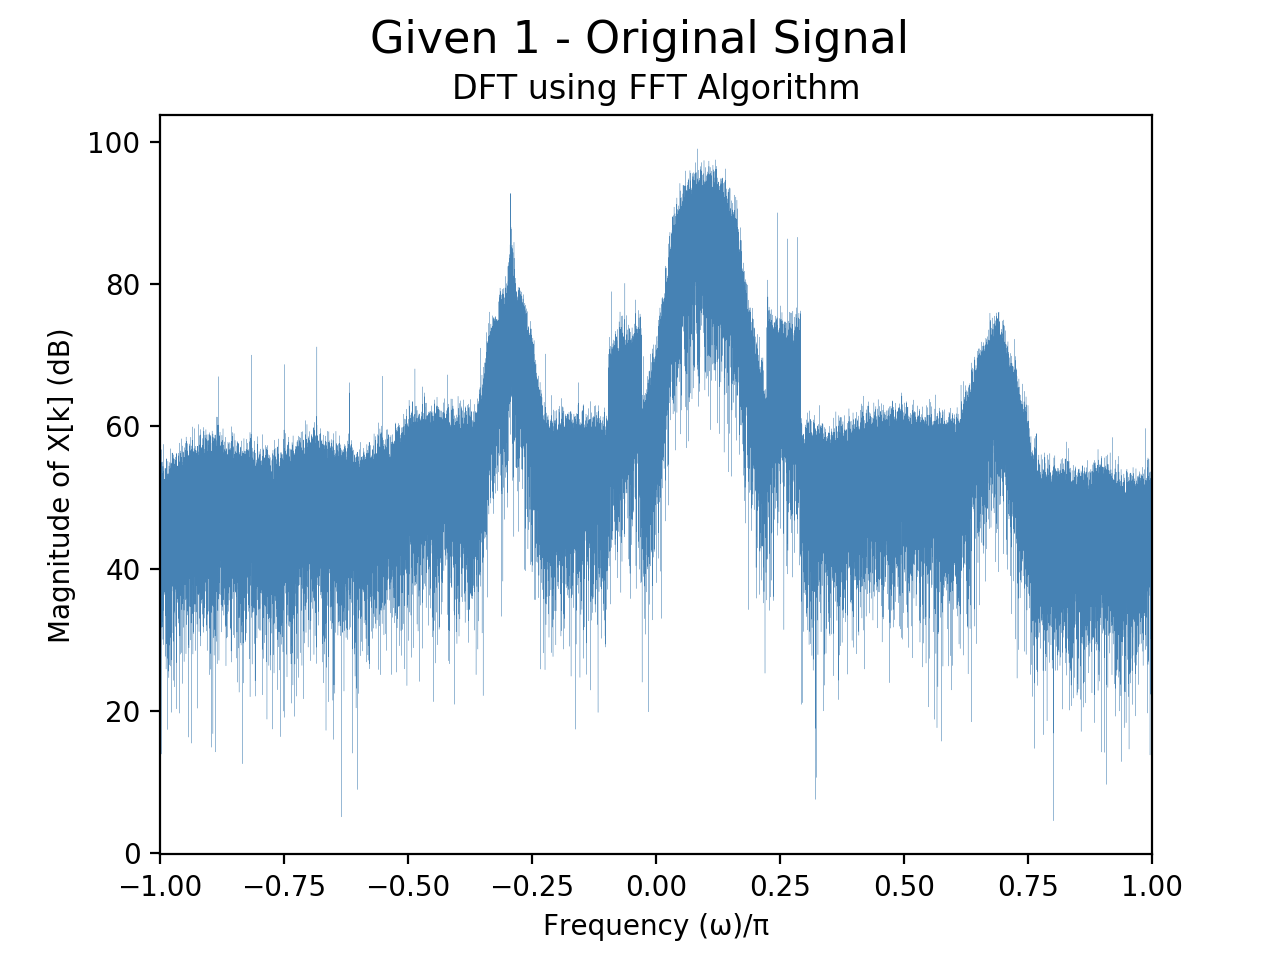
\includegraphics[width=.5\textwidth]{Figure_1.png}
    \caption{This is one of the original test signals given to us. It's parameters are listed in the raw data section. The plot represents what I expect.}
\end{figure}

\subsubsection{Modulation}

To modulate a component of the frequency domain into baseband, we first need to identify the appropriate complex exponential to multiply with the original signal. Each of my input signals was sampled at $f_s = 2048000$ Hz or $f_s = 2.048$ MHz. Reworded, our continuous signal has been converted to a discrete signal through sampling; we have done C/D conversion. We know that the output of a C/D converter can be thought of as a time normalization of a continuous time signal, as shown below:
\begin{IEEEeqnarray}{rCl}
    \text{CT} &\leftrightarrow& \text{DT} \\
    t &\leftrightarrow& n\\
    1 &\leftrightarrow& T
\end{IEEEeqnarray}

This also means we have frequency normalization, as shown below:
\begin{IEEEeqnarray}{rCl}
    \text{CT} &\leftrightarrow& \text{DT} \\
    \Omega_s &\leftrightarrow& 2\pi\\
    \Omega &\leftrightarrow& \omega
\end{IEEEeqnarray}

We can the identify $\omega_0$ for each signal through the following set of steps.

\begin{enumerate}[label=(\roman*), leftmargin=*, itemsep=0.4ex, before={\everymath{\displaystyle}}]%
  \item $\dfrac{\Omega_s}{\Omega_0} = \dfrac{2\pi}{\omega_0}$, where we map $\Omega_s$ to $2\pi$
  \item $\omega_0 = \dfrac{2\pi\Omega_0}{\Omega_s}$, where we solve for $\omega_0$
\end{enumerate}

Fig~\ref{fig:modulate} shows the process of modulation. It represents what I expect.

\begin{figure}[h] \label{fig:modulate}
    \centering
    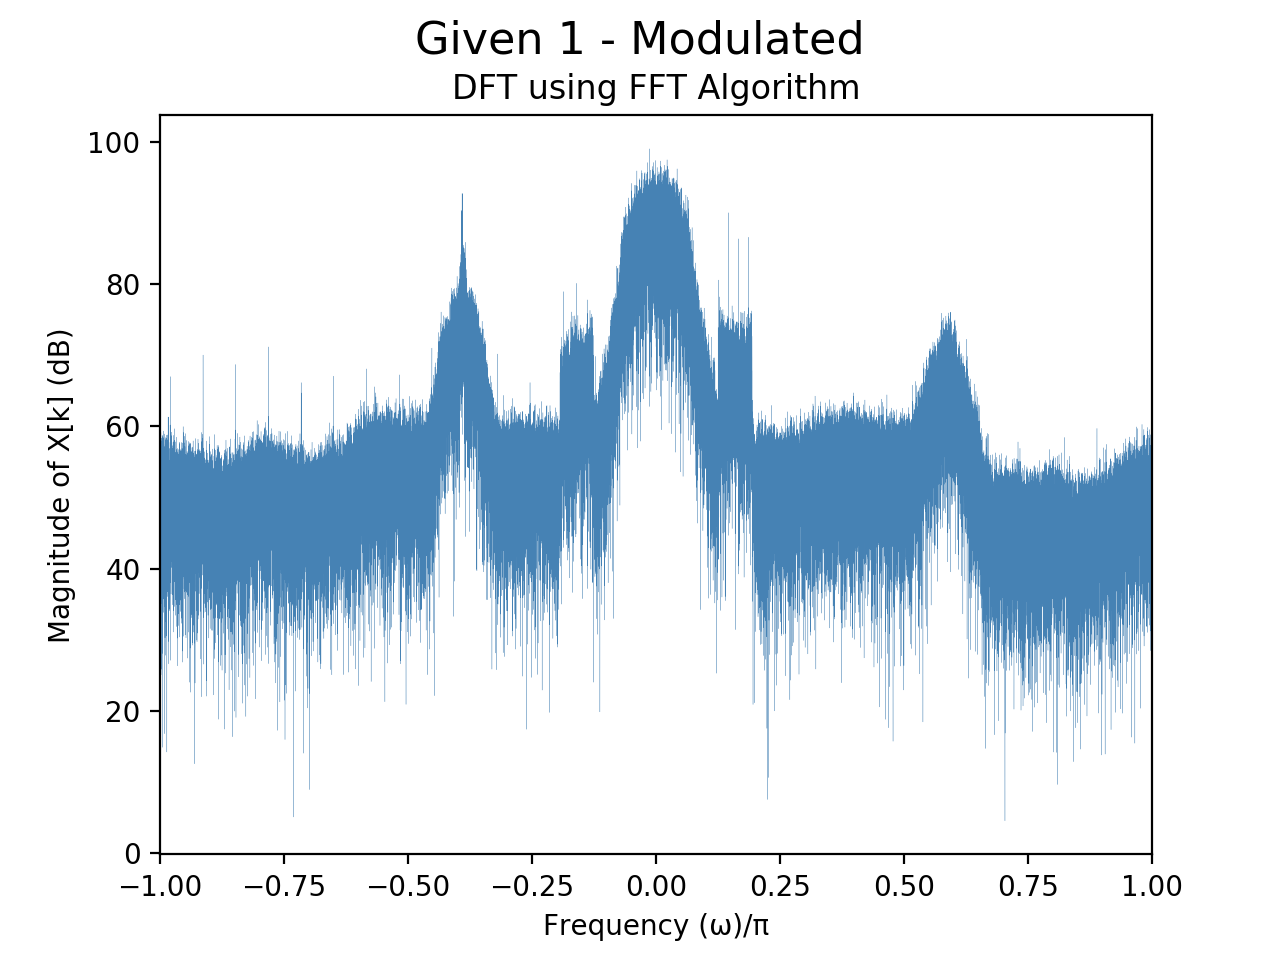
\includegraphics[width=.5\textwidth]{given_1_modulate.png}
    \caption{This plot show samples of the DTFT. This is following the modulation step, and the sound content shifted to an expected location - centered around 0. Therefore, this represents what I expect.}
\end{figure}

\subsubsection{Downsampling} \label{sec:downsampling_1}

Following modulation, I implemented a downsampler. To prevent aliasing, I designed an anti-aliasing filter. The pivotal aspect of design here is the choice of the cutoff frequency. First, let's identify some relevant values:
\begin{IEEEeqnarray}{rCl}
    f_s &=& 2.048 \text{ MHz}\\
    \Omega_s &=& \dfrac{2\pi}{f_s}\\
    M &=& 8\\
\end{IEEEeqnarray}
Frequency scaling from decimation impacts the frequency representation as follows:
\begin{IEEEeqnarray}{rCl}
    X(e^{j\omega}) &=& \dfrac{1}{T_1} \sum\limits_{k = -\infty}^{\infty}X_c\left(j\left(\dfrac{\omega}{T_1}-\dfrac{2\pi k}{T_1}\right)\right) \\
    X_d(e^{j\omega}) &=& \dfrac{1}{M} \sum\limits_{i = 0}^{M-1}X\Big(e^{j\left(\dfrac{\omega}{M}-\dfrac{2\pi i}{M}\right)}\Big)
\end{IEEEeqnarray}
We know that discrete-time decimation results in periodic repetitions and frequency scaling in the frequency domain. We want to prevent aliasing, so our cutoff frequency should prevent overlap from these shifted replicas. The relationship between $X(e^{j\omega})$ and $X(e^{j\omega})$ shows this.

To prevent aliasing, we set the discrete time cutoff frequency, $\omega_c$, to equal $\pi/8$. I then chose appropriate parameters to implement this filter. I chose to use a Chebyshev Type II filter for the following reasons: 1) it has a flat magnitude response in the passband which is important for audio signal filtering, and 2) while there are ripples in the stopband and less stopband attenuation, the Chebyshev Type II maximizes the rate of cutoff between the passband and the stopband. Following the choice of desirable filter parameters, I used functions from the python \code{signal} package to optimize for the appropriate Chebyshev filter parameters. I chose to set $\omega_s = \omega_c$ because I wanted to prevent aliasing entirely. I understand that this may prevent some relevant signal content from coming through. $\omega_p$ was then chosen through consideration of the trade off between filter order and transition width. $\omega_s - .1\omega_s$ seemed appropriate and produced decent results.
% I chose the function \code{signal.remez} from the \code{scipy.signal} package to build the low pass filter.

\paragraph{Chebyshev II Parameters}
\begin{enumerate}
    \item Discrete-time Cutoff Frequency $\omega_c = \dfrac{\pi}{8}$
    \item Equivalent Continuous-Time Cutoff Frequency $\Omega_c = \dfrac{\omega_c\Omega_s}{2\pi}$
    \item Discrete-time passband edge: $\omega_{pass} =  \dfrac{2\pi\Omega_{pass}}{\Omega_s} $
    \item Discrete-time stopband edge: $\omega_{stop} = \dfrac{\pi}{8}$
    \item Equivalent continuous-time passband edge: $\Omega_{pass} = \Omega_{stop} - .1\Omega_{stop}$
    \item Equivalent continuous-time stopband edge: $\Omega_{stop} = \dfrac{\omega_{stop}\Omega_s}{2\pi}$
    \item Maximum gain in the passband: 0 dB.
    \item Minimum gain in the passband: -1 dB.
    \item Maximum gain in the stopband: -50 dB
\end{enumerate}

\begin{figure}[h] \label{fig:chebII}
    \centering
    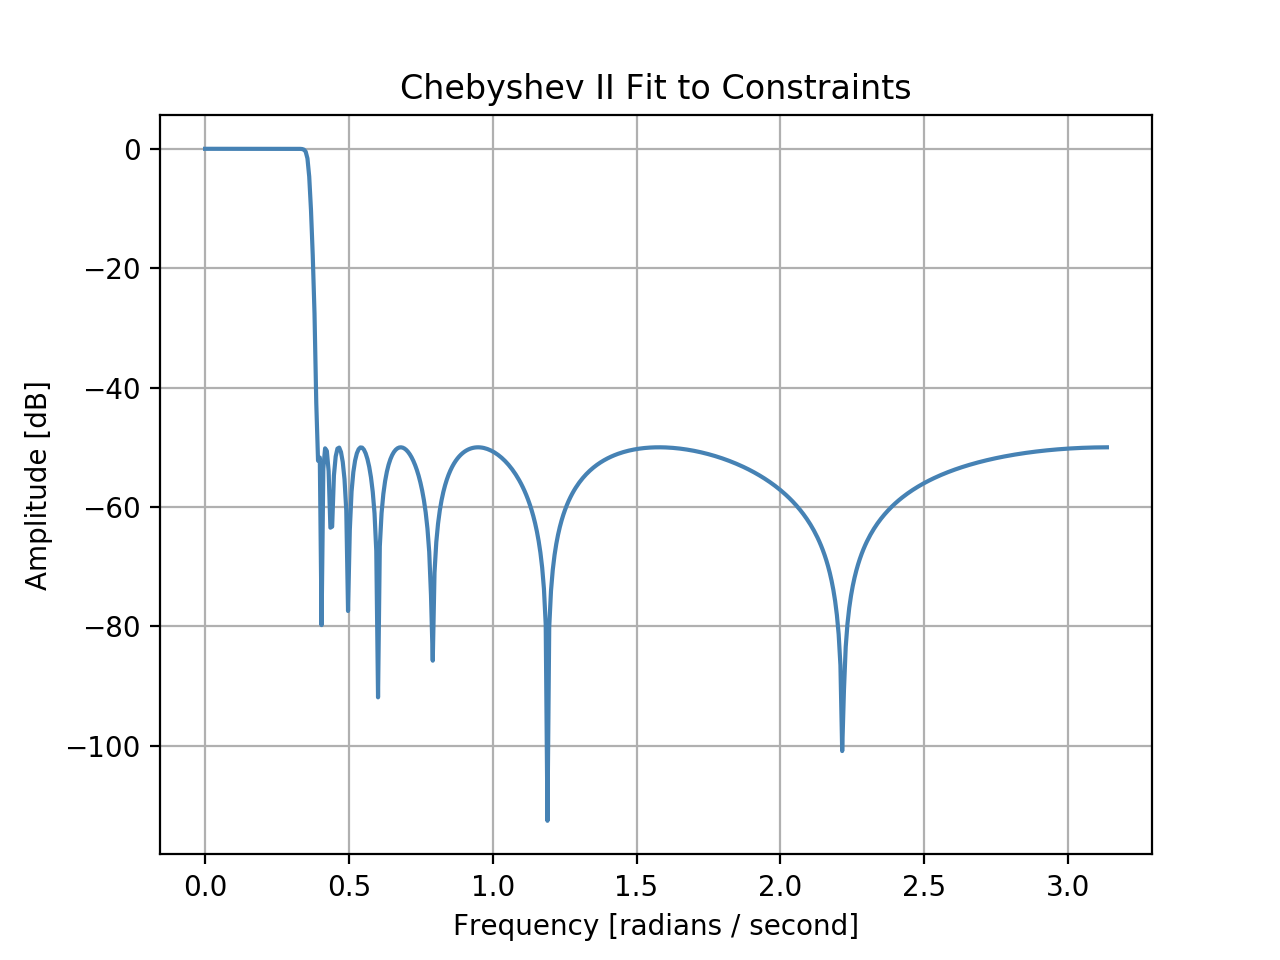
\includegraphics[width=.5\textwidth]{kaiser_1.png}
    \caption{This is the frequency response of the Chebyshev II filter designed for the above specifications. This represents what I expect.}
\end{figure}

\begin{figure}[h] \label{fig:chebII}
    \centering
    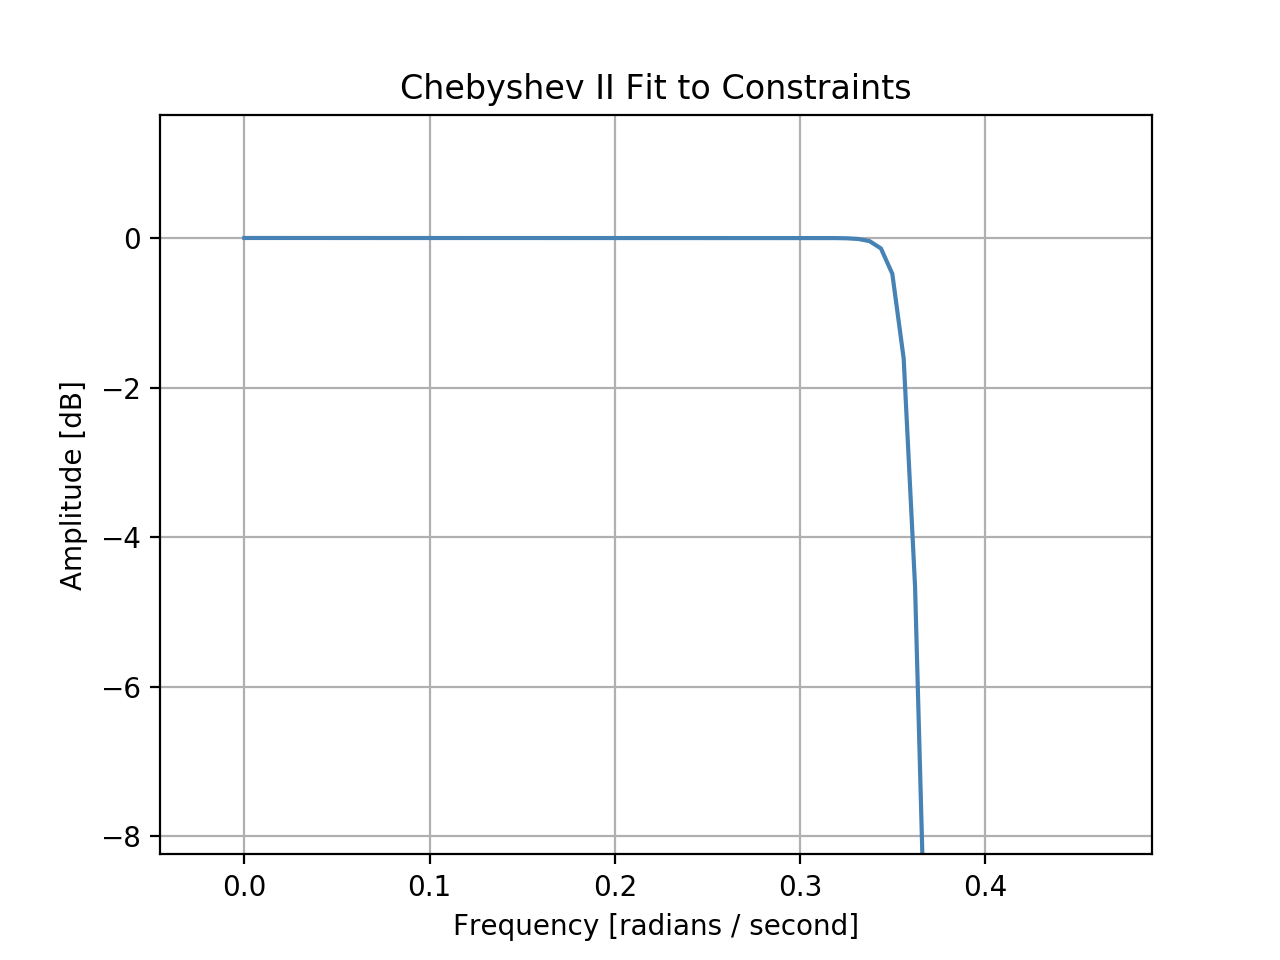
\includegraphics[width=.5\textwidth]{kaiser_2.png}
    \caption{This is the passband of the frequency response of the Chebyshev II filter designed for the above specifications. This represents what I expect.}
\end{figure}

\begin{figure}[h] \label{fig:chebII}
    \centering
    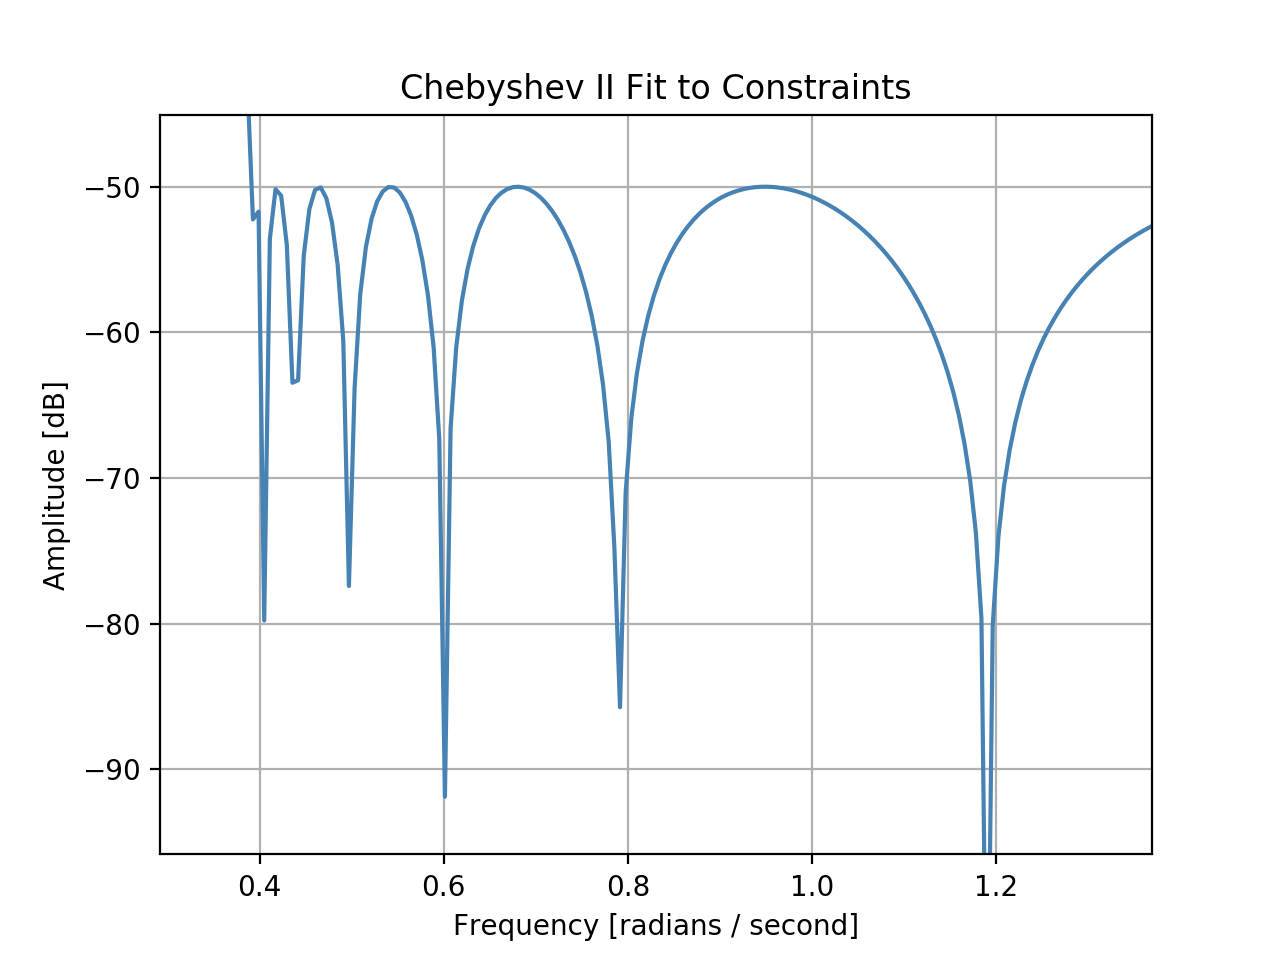
\includegraphics[width=.5\textwidth]{kaiser_3.png}
    \caption{This is the passband of the frequency response of the Chebyshev II filter designed for the above specifications. This represents what I expect.}
\end{figure}

I first chose to use infinite-impulse response (IIR) filter design techniques because they produce lower order systems. I recognize that with a polyphase implementation, FIR would be more desirable as computational complexity is reduced and linear phase may be achieved. Following implementation of the IIR filter, it was clear that improvements could be made in sound quality to output signal. So, a FIR lowpass filter using the Parks-McClellan algorithm was built. Without polyphase implementation, I saw that I could still perform filtering even with a higher order system. I chose Parks-McClellan because it efficiently compute the optimal filter for given parameters when considering an optimality criterion of minimum maximum error in the passband(s) and stopband(s). Just as in our Week 6 homework, we designed three parameters to correct for the inconsistency between IIR and FIR design procedures. Because I chose equivalent parameters for Maximum gain in the passband, minimum gain in the passband, and maximum gain in the stopband, I maintained the same values derived from Homework 6.

\paragraph{Parks-McClellan Parameters}
\begin{enumerate}
    \item Discrete-time Cutoff Frequency $\omega_c = \dfrac{\pi}{8}$
    \item Equivalent Continuous-Time Cutoff Frequency $\Omega_c = \dfrac{\omega_c\Omega_s}{2\pi}$
    \item Discrete-time passband edge: $\omega_{pass} =  \dfrac{2\pi\Omega_{pass}}{\Omega_s} $
    \item Discrete-time stopband edge: $\omega_{stop} = \dfrac{\pi}{8}$
    \item Equivalent continuous-time passband edge: $\Omega_{pass} = \Omega_{stop} - .1\Omega_{stop}$
    \item Equivalent continuous-time stopband edge: $\Omega_{stop} = \dfrac{\omega_{stop}\Omega_s}{2\pi}$
    \item Maximum gain in the passband: 0 dB.
    \item Minimum gain in the passband: -1 dB.
    \item Maximum gain in the stopband: -50 dB
    \item Gain parameter: $k \approx .94563 $
    \item Adjusted passband parameter: $\delta^{(pb)}_{FIR} \approx .0575$
    \item Adjusted stopband parameter: $\delta^{(pb)}_{FIR} \approx 1/(100k\sqrt{10})$
\end{enumerate}

\begin{figure}[h] \label{fig:parks_1}
    \centering
    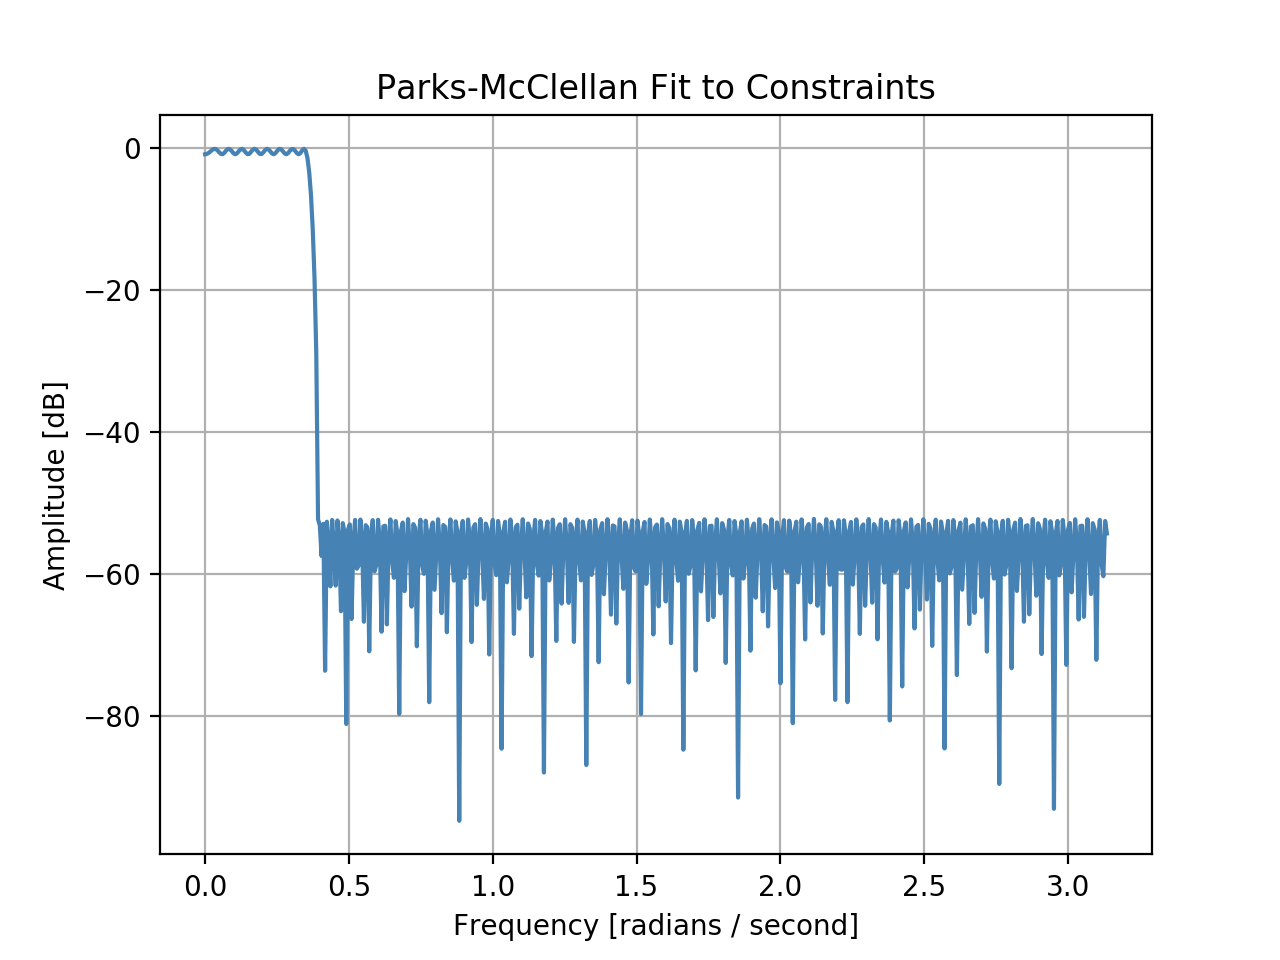
\includegraphics[width=.5\textwidth]{given_1_parks_1.png}
    \caption{This is the frequency response of the Parks-McClelland filter designed for the above specifications. This represents what I expect.}
\end{figure}

\begin{figure}[h] \label{fig:parks_2}
    \centering
    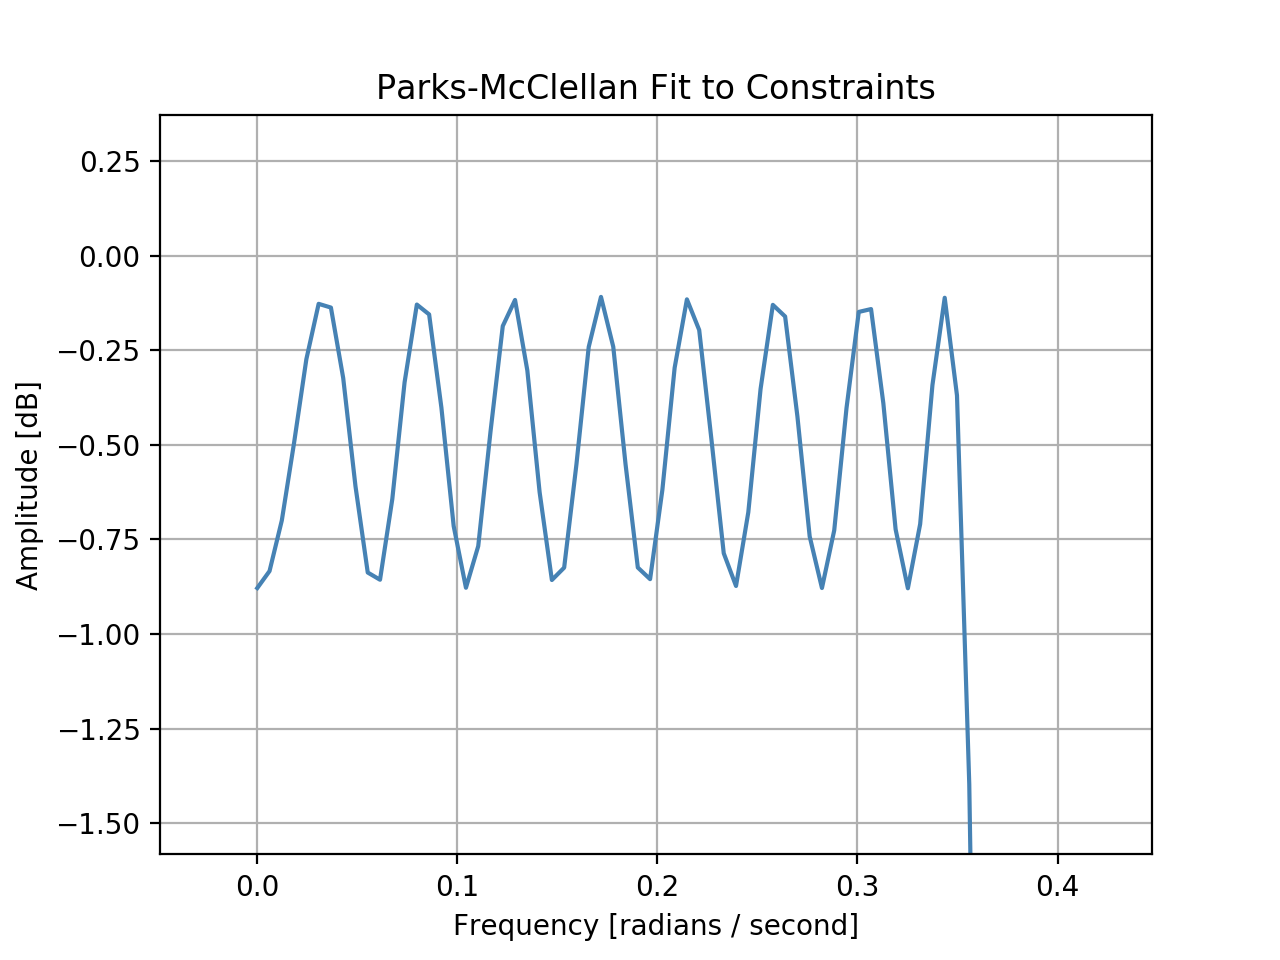
\includegraphics[width=.5\textwidth]{given_1_parks_2.png}
    \caption{This is the passband of the frequency response of the Parks-McClelland filter designed for the above specifications. This represents what I expect.}
\end{figure}

\begin{figure}[h] \label{fig:parks_3}
    \centering
    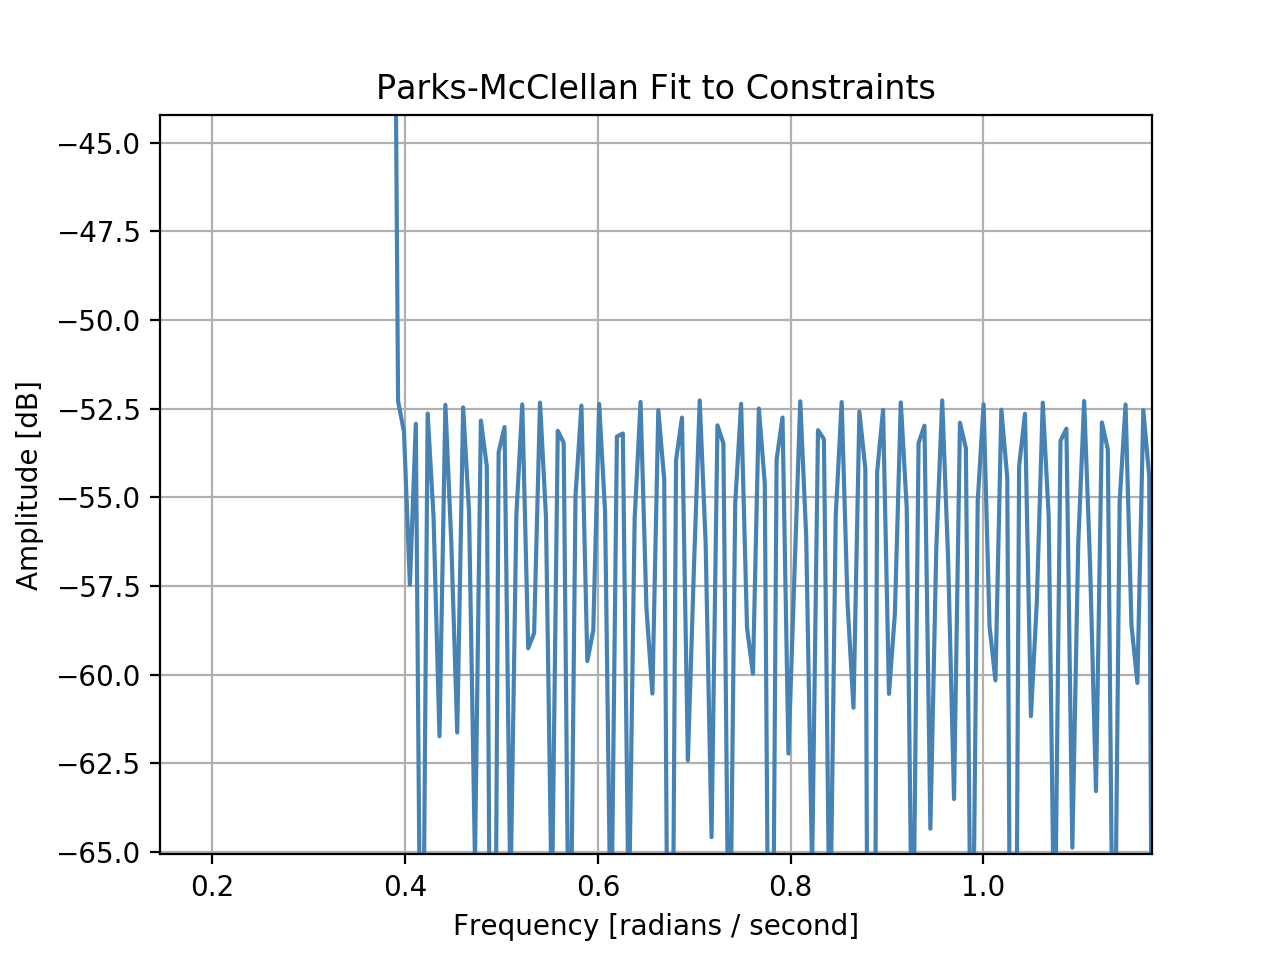
\includegraphics[width=.5\textwidth]{given_1_parks_3.png}
    \caption{This is the stopband of the frequency response of the Parks-McClelland filter designed for the above specifications. This represents what I expect.}
\end{figure}

Following implementation of the anti-aliasing filter, I took every eighth sample from the time-domain representation of the signal which is equivalent to decimation. Analysis of the DFT showed results which aligned with my expectations, as decimation produces frequency expansion.

\begin{figure}[h] \label{fig:decimation_8}
    \centering
    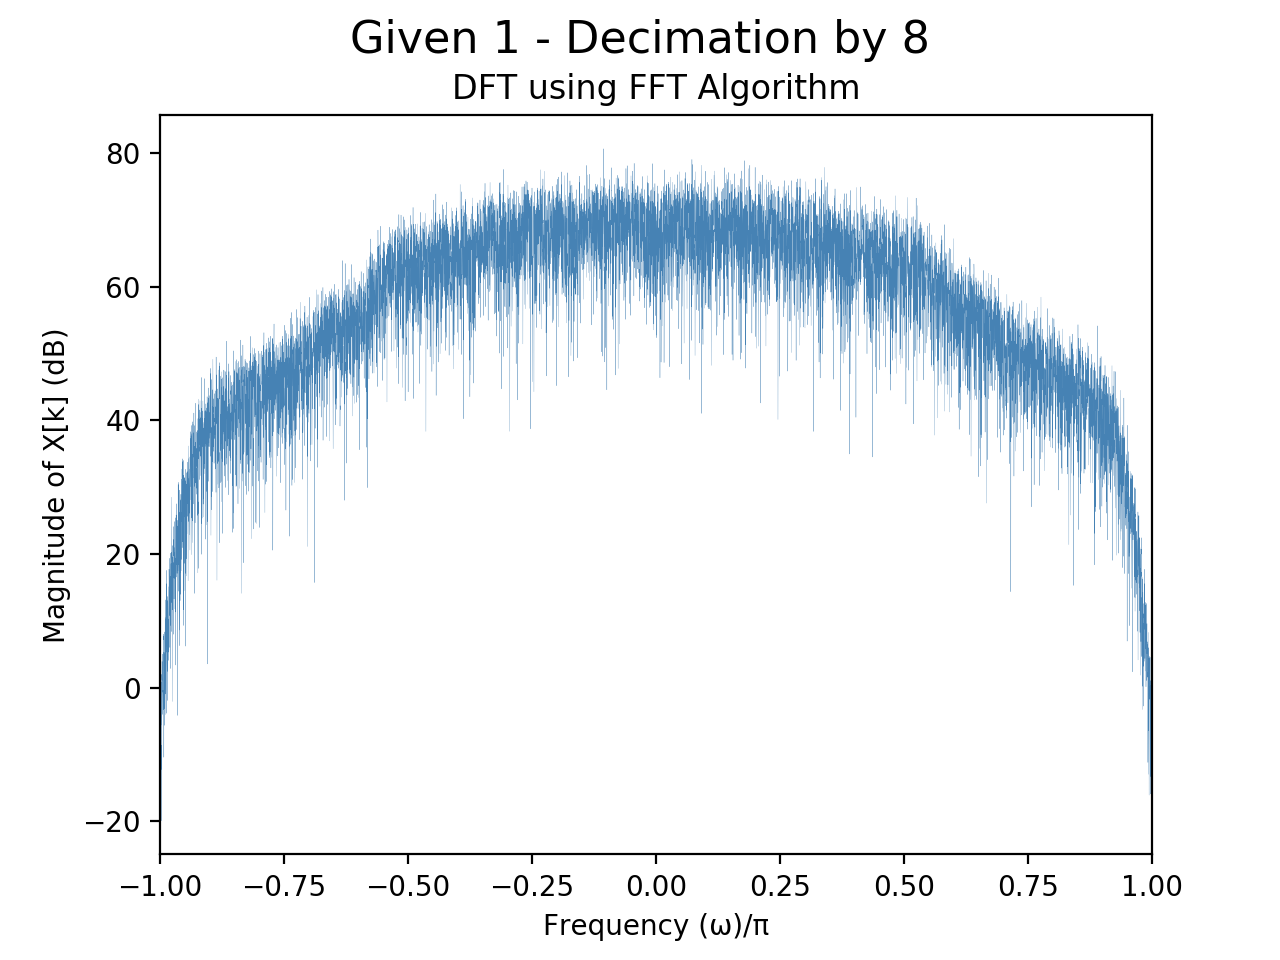
\includegraphics[width=.5\textwidth]{given_1_decimation_by_8.png}
    \caption{This plot show samples of the DTFT. This is following the decimation by 8 step. We see frequency expansion and, thus, this represents what I expect.}
\end{figure}

\subsection{FM Demodulation}

Now that we have modulated the frequency content down to baseband, we performed FM demodulation. This extracts the real-valued mono audio signal from the complex baseband signal. We refer back to the section exploring the raw data, Section~\ref{sec:raw_data}, as this points to the motivation for each of these steps.

\subsubsection{Frequency Discriminator}

We developed a frequency discriminator. Out of the frequency discriminator, we will produced the derivative of the phase of our input signal. This involved three major steps.

First, we implemented the limiter step, and normalized our input through the following equation:
\begin{IEEEeqnarray}{rCl}
    y_1[n] = \dfrac{y_[n]}{\abs{y_[n]}}
\end{IEEEeqnarray}
Next, we designed an FIR discrete time differentiator to produce $y_{1a}$. We wanted to obtain samples of the derivative of the bandlimited interpolation of the input signal, $y_1$. First, we identified the continuous time transfer function of a differentiator. This is as follows:
\begin{IEEEeqnarray}{rCl}
    H(j\Omega) = j\Omega
\end{IEEEeqnarray}
We find the equivalent discrete time system which will produce output samples equivalent to samples of the bandlimited interpolation of the discrete time signal, or samples of the derivative of the equivalent continuous-time signal. This discrete-time system is as follows:
\begin{IEEEeqnarray}{rCl}
    H_{diff}(e^{j\omega}) &=& \dfrac{j\omega}{T}\\
    T &=& \dfrac{1}{f_s}
\end{IEEEeqnarray}
We omit the $1/T$ factor as inclusion of this leads to extreme gain and severe sound output quality distortion. To implement an ideal discrete time differentiator with linear phase, we use:
\begin{IEEEeqnarray}{rCl}
    H_{diff}(e^{j\omega}) = (j\omega)e^{-j\omega M/2}
\end{IEEEeqnarray}
To realistically use this discrete-time differentiator, we implemented the time-domain representation of this transfer function and used a Kaiser window design procedure to achieve a realizable impulse response. The time-domain representation is as follows:
\begin{IEEEeqnarray}{rCl}
    h_{diff}[n] = \dfrac{cos(\pi(n-M/2)}{(n-M/2} - \dfrac{sin\pi(n-M/2)}{\pi(n-M/2)^2}, \text{ where } 0 \leq n \leq M + 1
\end{IEEEeqnarray}
The Kaiser window significantly outperforms Bartlett, Hanning, Hamming, and Blackman window. This is most apparent when considering approximation error vs. transition width. The Kaiser window has two parameters: filter length ($M+1$), and a shape parameter ($\beta$). We choose the following Kaiser window Parameters:

\paragraph{Kaiser Window Design}
\begin{enumerate}
    \item $M = 5$ ($Length = M + 1$)
    \item $\beta = 2.4$
\end{enumerate}

We generated a vector, $n$ matching the length of our designed window as stated above. It can be shown that multiplying $h_{diff}[n]$ by a symmetric window of length (M+1) will result in a type III or type IV generalized linear-phase system. This is also apparent in the plot of the windowed impulse response in Fig~\ref{fig:window-diff}. We choose a type IV generalized linear-phase system, (verified by our chosen parameters), as the lack of constraining H(z) to have a zero at $z = -1$ produces less significant error. Although this produces a non-integer delay, compensating for this is quite simple.

\begin{figure}[h] \label{fig:differentiator}
    \centering
    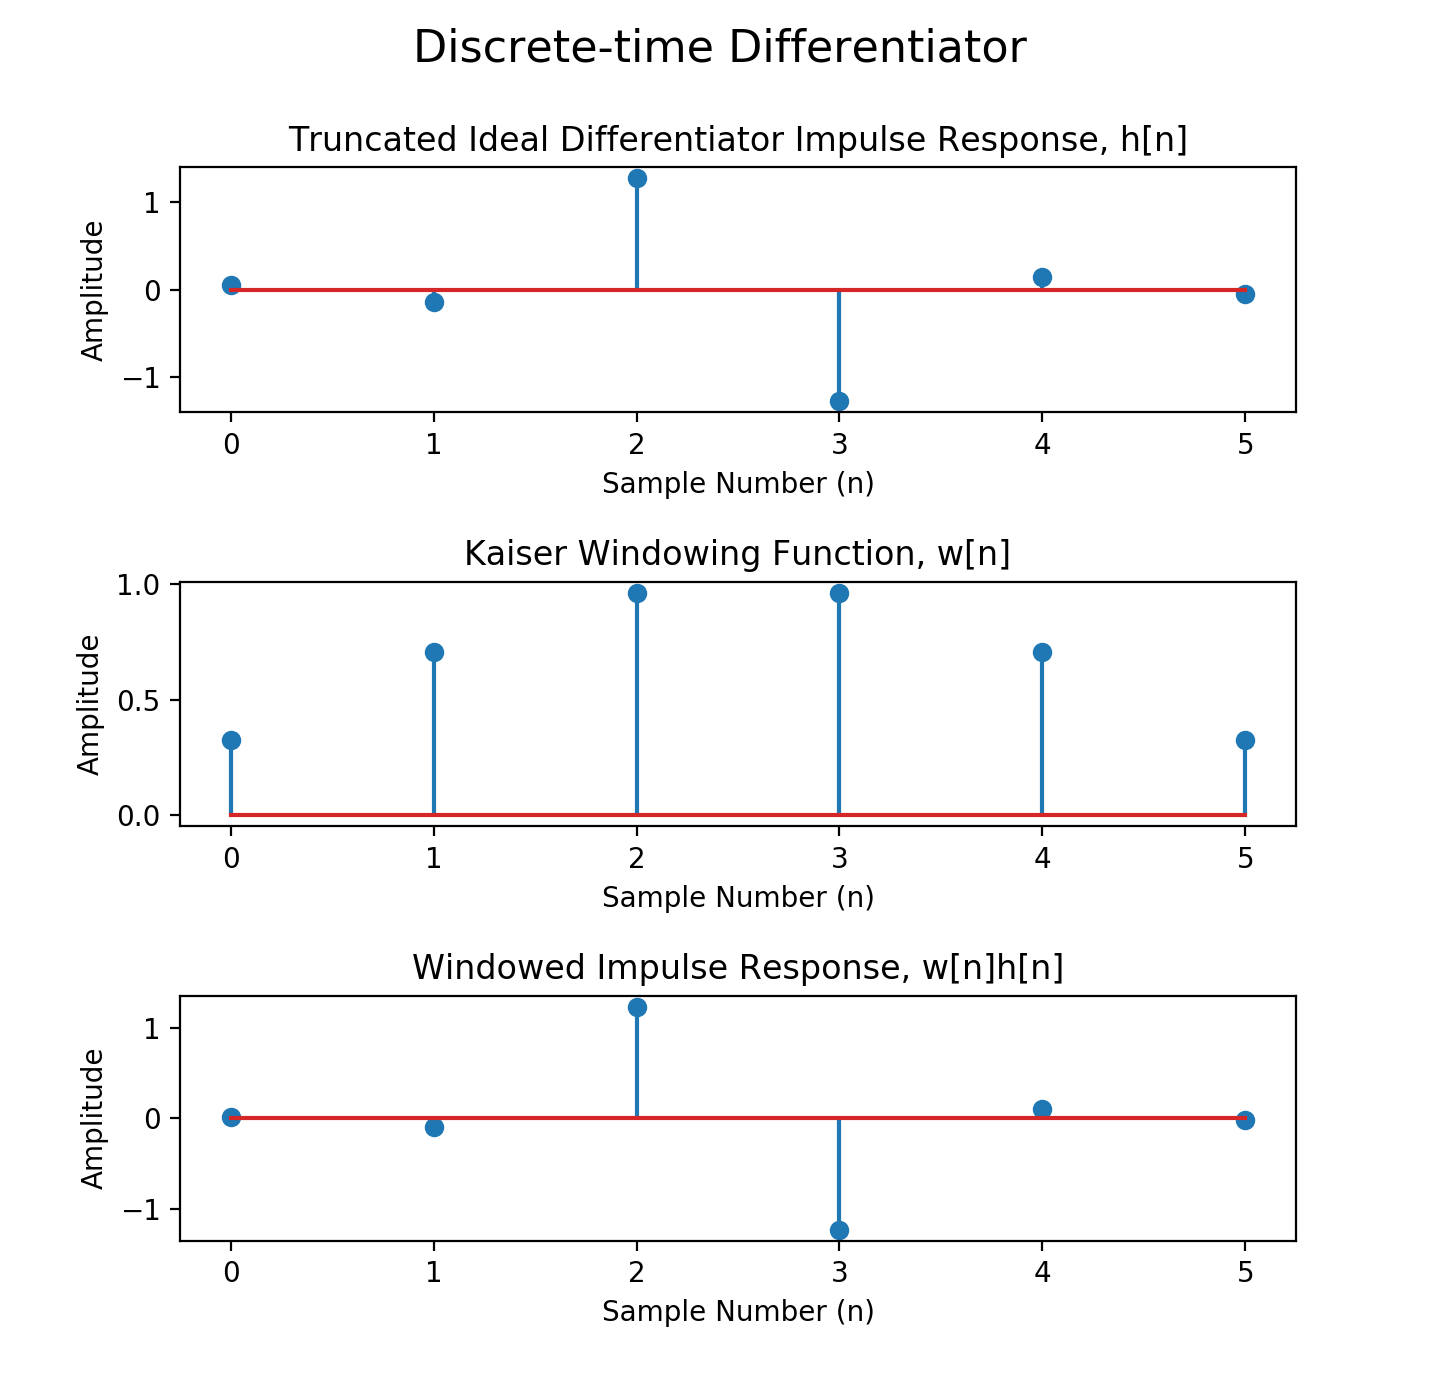
\includegraphics[width=.5\textwidth]{differentiator.png}
    \caption{This is the time domain representation of the designed discrete-time differentiator showing the windowing procedure used. This resembles an impulse response of a differentiator so it is what I expect.}
\end{figure}

Next, we implemented conjugation of $y_1$ through the feedforward path of our discriminator diagram, and implemented a delay block matching the group delay of our designed linear phase differentiator. Similar to how we derived the transfer function of the differentiator, we found the discrete-time function which samples the bandlimited interpolation of the discrete-timne signal at noninteger sample positions. This led to the following transfer function:
\begin{IEEEeqnarray}{rCl}
    h_{nid}[n] = \dfrac{sin\pi(n-\Delta)}{\pi(n-\Delta)}, \text{ where } 0 \leq n \leq M + 1
\end{IEEEeqnarray}
We implement a rectangular windowed version of this of length $M+1$, as it was quite straightforward to do and did not reduce quality of our final output signal. So, this signal was convolved with the conjugate of $y_1$ which gives us $y_{1b}$.

We then multiply $y_{1a}$ and $y_{1b}$ to get $y_2$. Finally, we took to imaginary component of the signal.

\begin{figure}[h] \label{fig:discriminator}
    \centering
    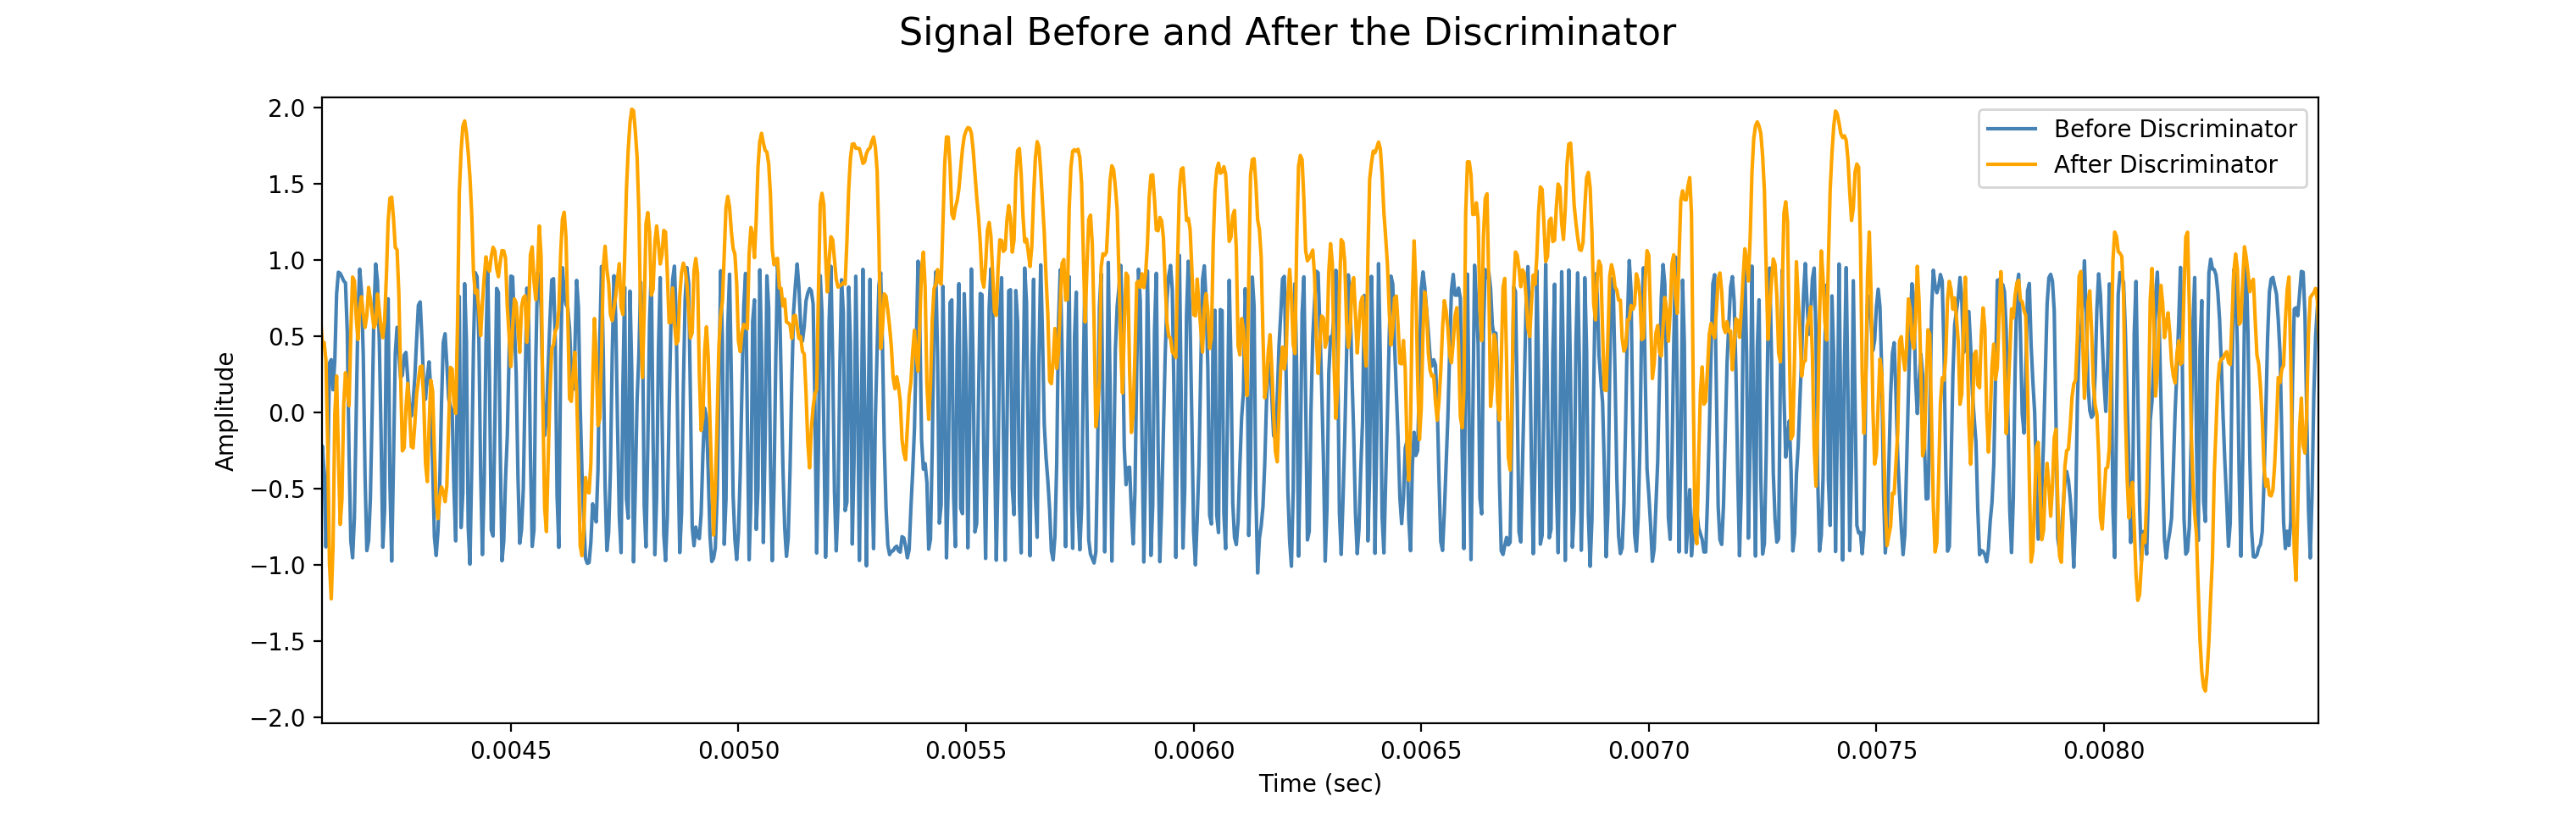
\includegraphics[width=\textwidth]{given_1_discriminator_time.png}
    \caption{This is a comparison of the input of the discriminator to its output. We see clear frequency modulation to amplitude modulation. This is what I expect.}
\end{figure}

\begin{figure}[h] \label{fig:discriminator_2}
    \centering
    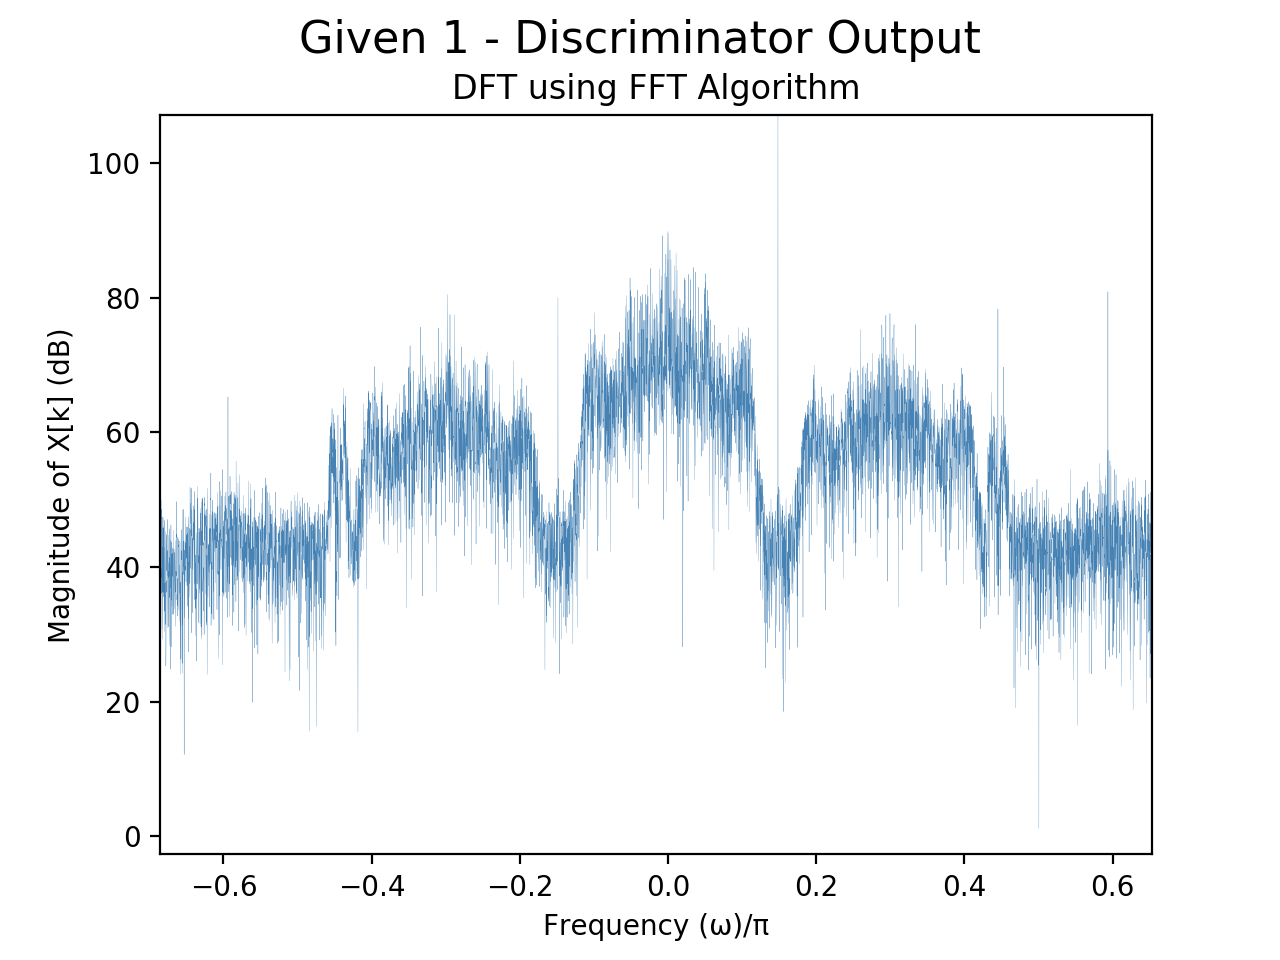
\includegraphics[width=.5\textwidth]{given_1_discriminator.png}
    \caption{This is the output from the discriminator. I see a signal which is symmetric, so I know that I got a real-valued signal. This is expected. It is also clear that we distinguished multiple frequency components from the previous signal. This is what I expect from a discriminator.}
\end{figure}

\subsubsection{Deemphasis Filter}

Next, we implemented a deemphasis filter. We were given the following continuous-time filter:
\begin{IEEEeqnarray}{rCl}
    H(j\Omega) = \dfrac{1}{1 + j\Omega\tau_d}
\end{IEEEeqnarray}
We chose to implement the given continuous time filter in discrete time through use of the bilinear transformation. The bilinear transformation was chosen over the impulse invariance method for its desirable characteristics not limited to mapping stable continuous-time poles to stable discrete-time poles, and that it is an algebraic transformation. No prewarping was necessary which was determined as use of prewarping did not produce noticeable impact on the output sound quality. To do this, we substituted $s$ for $j\Omega$, performed the transformation, and filtered the signal.

\begin{figure}[h] \label{fig:deemphasis_1}
    \centering
    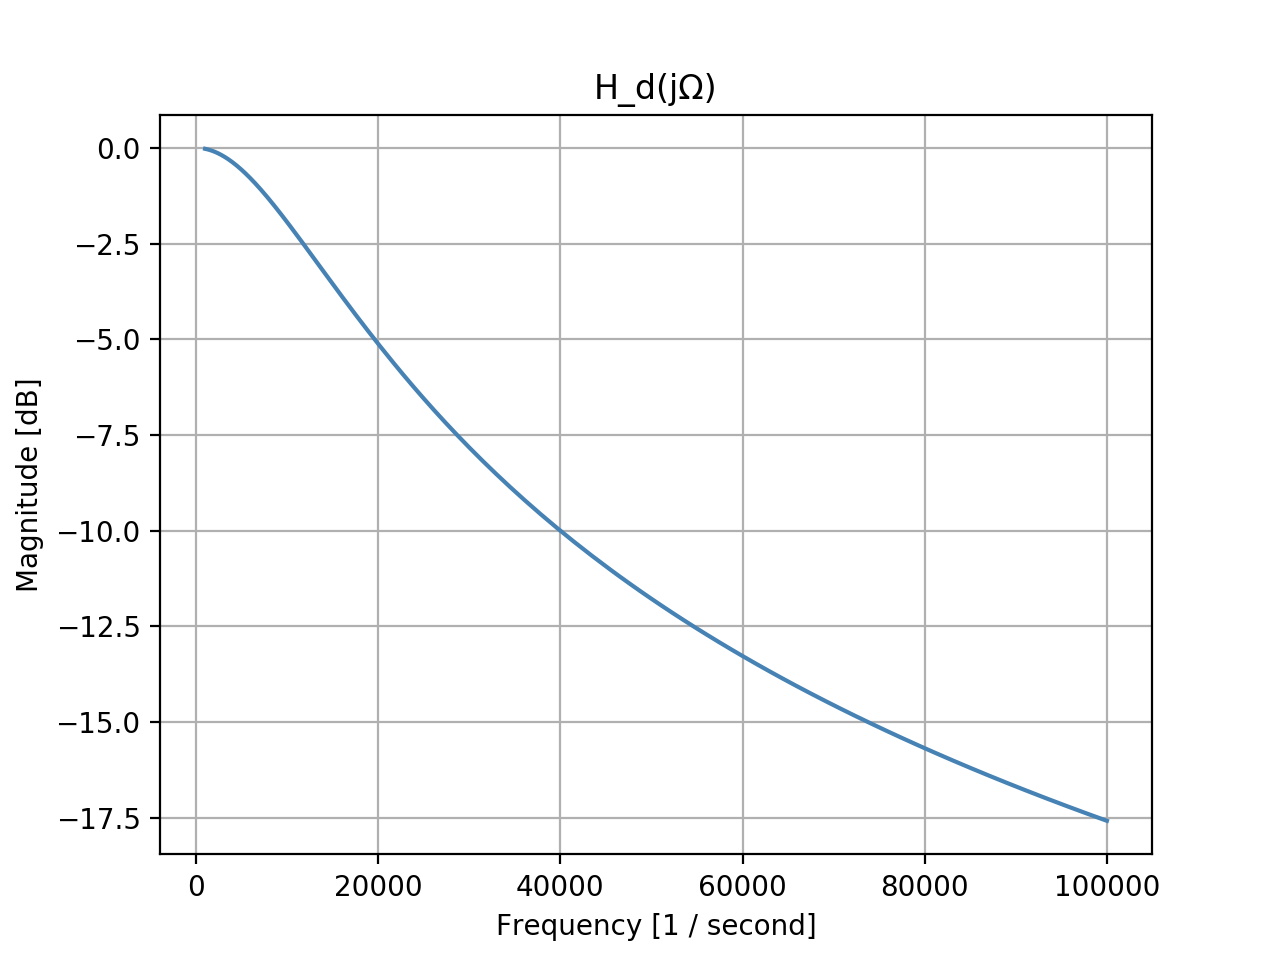
\includegraphics[width=.5\textwidth]{h_d.png}
    \caption{This is the frequency response plot of the deemphasis filter. From my knowledge of bode plot drawing, this represents what I expect.}
\end{figure}

\begin{figure}[h] \label{fig:deemphasis_2}
    \centering
    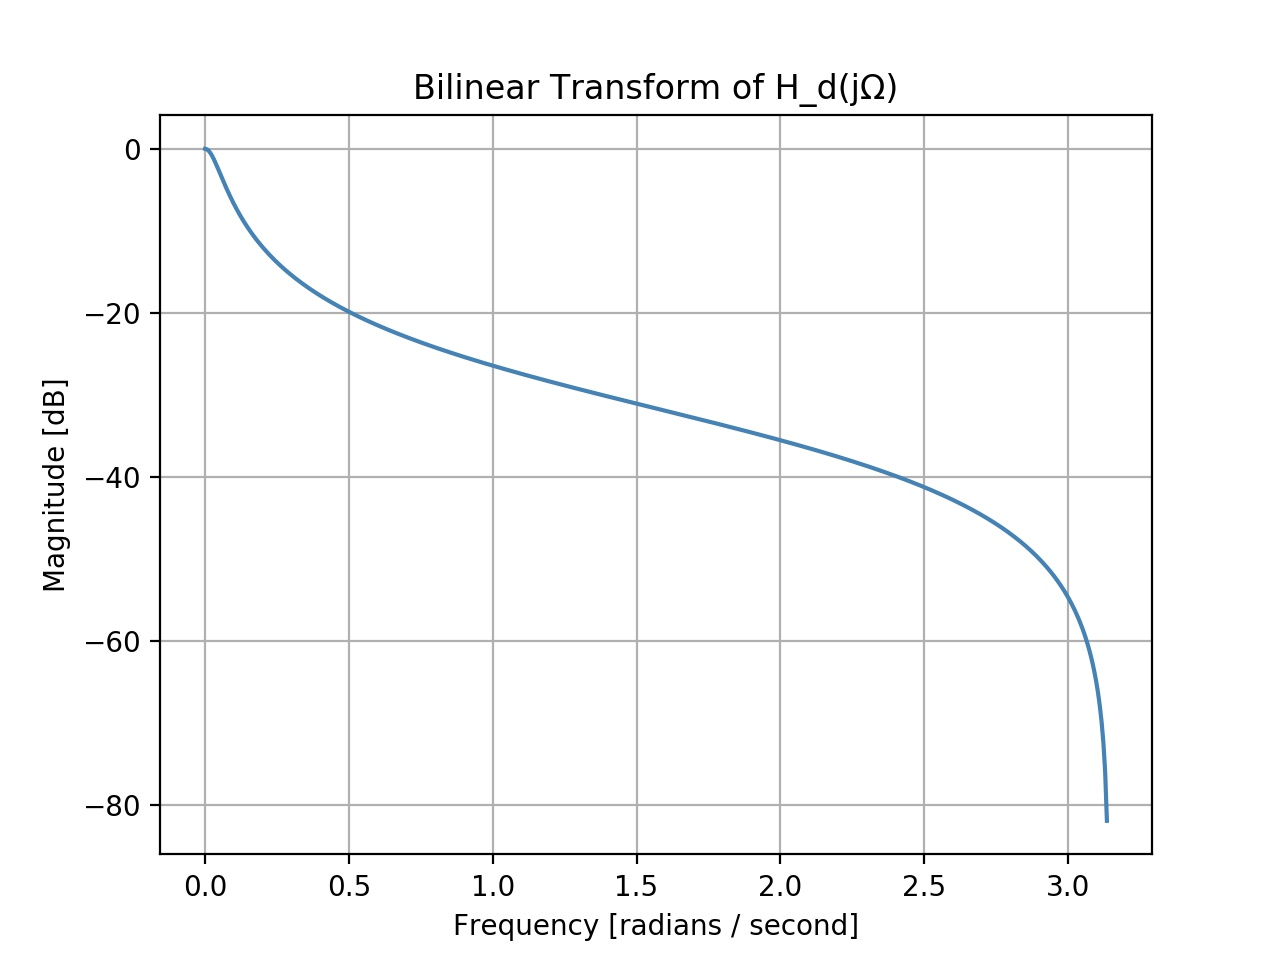
\includegraphics[width=.5\textwidth]{bilinear.jpg}
        \caption{This is the frequency response plot of the transformed deemphasis filter using the bilinear transform. From my knowledge of bode plot drawing, this represents what I expect. Because I did no prewarping, the shape of the response is also expected.}
\end{figure}

\begin{figure}[h] \label{fig:deemphasis_3}
    \centering
    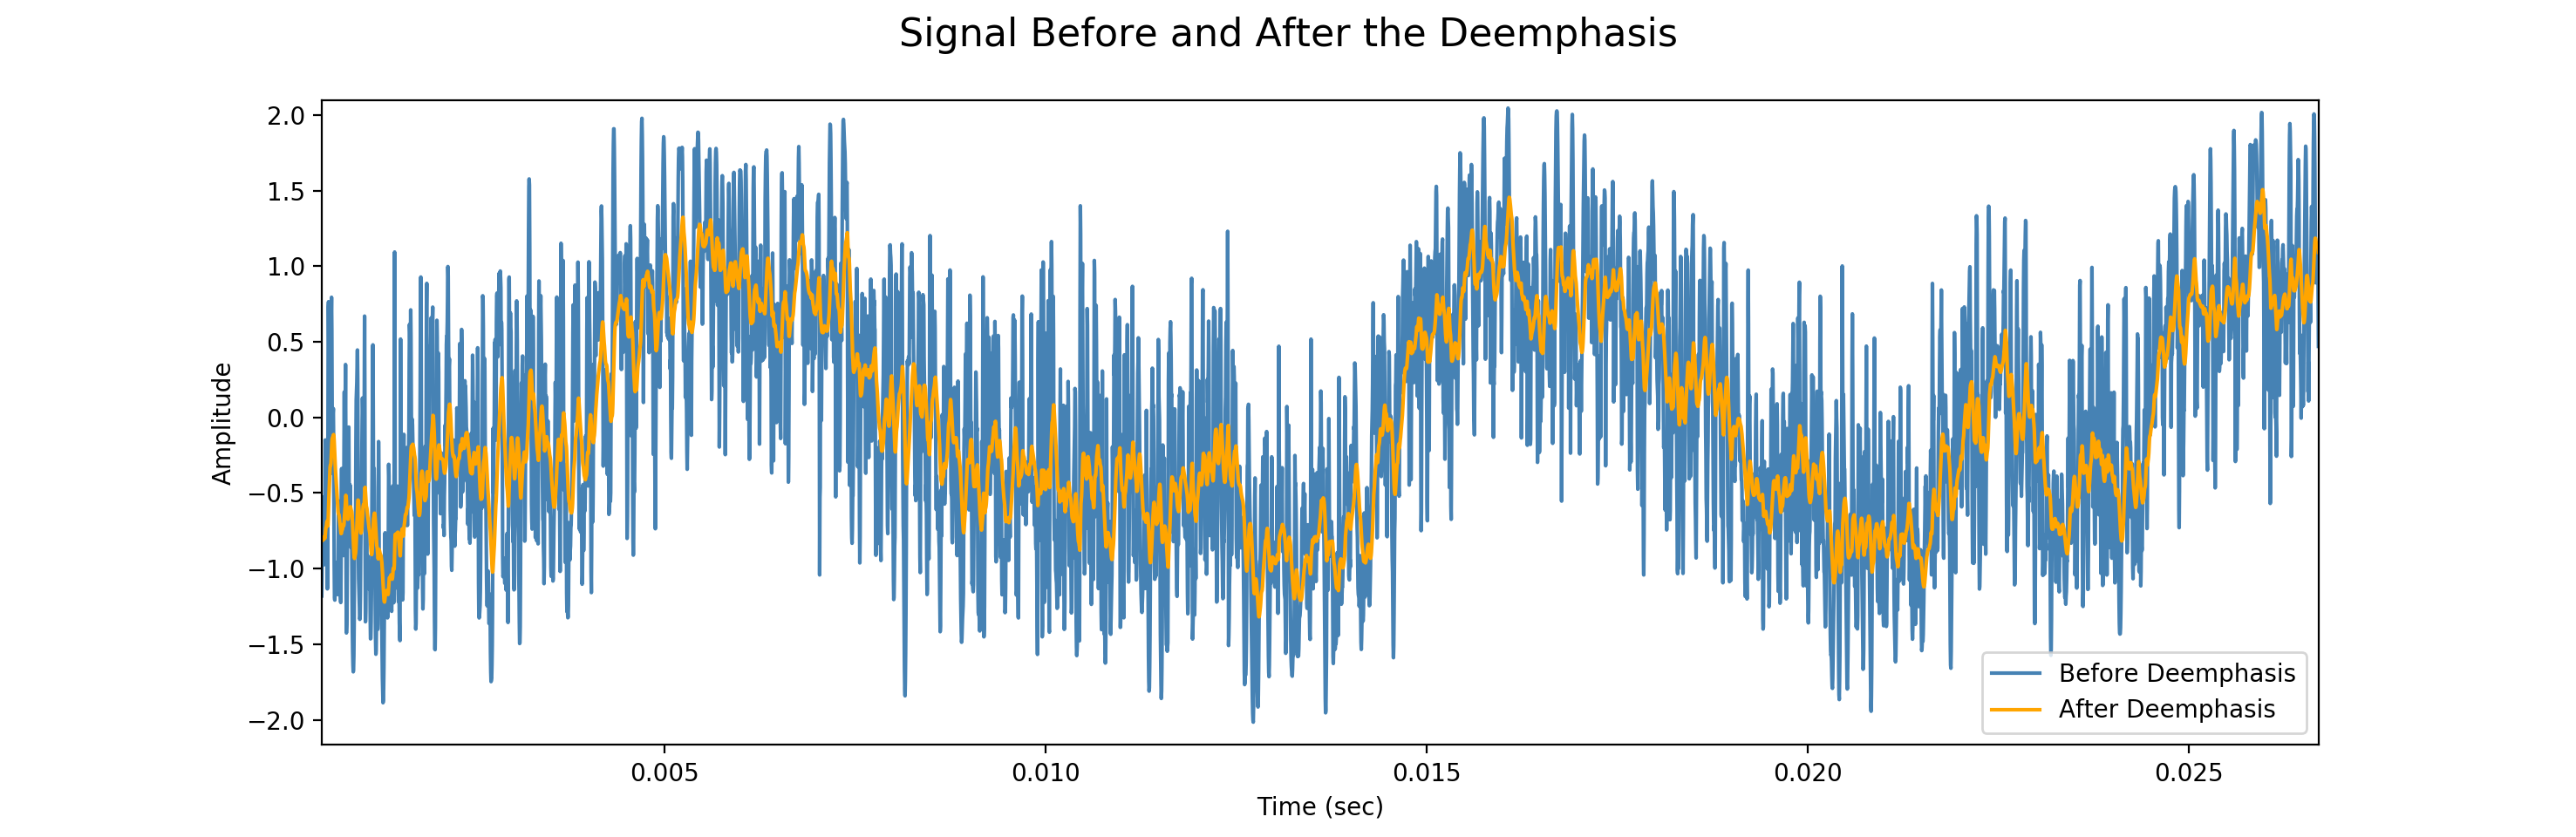
\includegraphics[width=\textwidth]{deemphasis.png}
    \caption{This is the comparison between the input to the deemphasis filter and the output. Because this filter accounts for the analog preemphasis used in radio communication, the shown input output relationship makes sense.}
\end{figure}

\begin{figure}[h] \label{fig:deemphasis_4}
    \caption{}
    \centering
    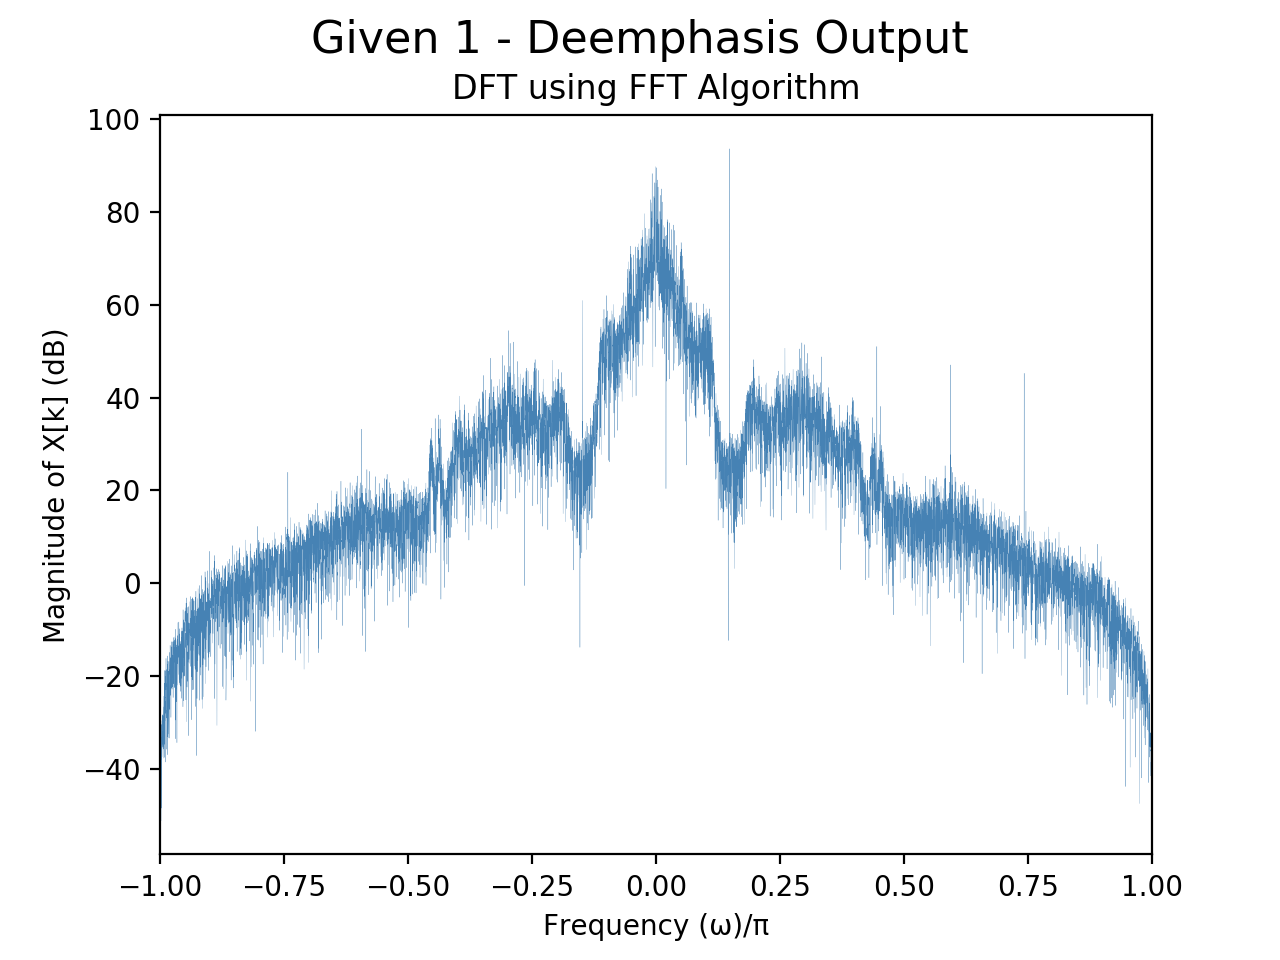
\includegraphics[width=.5\textwidth]{given_1_deemphasis.png}
    \caption{This is the frequency content of the output from the deemphasis filter. It clearly reduced the power of the frequency content outside of the band we are interested in.}
\end{figure}

\subsubsection{Lowpass Filter}

We next designed a lowpass filter account for the pilot tone at $19$ kHz, the stereo audio signal from $23$ to $38$ kHz, and message band for content information. 

The design procedure for this lowpass filter was identical to the design procedure for the anti-aliasing filter. Once again, a filter optimized through the Parks-McClellan algorithm was developed constrained to the filter parameters below. The sampling frequency $f_s'$ at this time was $256$ kHz

\paragraph{Parks-McClellan Parameters}
\begin{enumerate}
    \item Discrete-time passband edge: $\omega_{pass} =  \dfrac{2\pi\Omega_{pass}}{\Omega_s}$
    \item Discrete-time stopband edge: $\omega_{stop} =   \dfrac{2\pi\Omega_{stop}}{\Omega_s}$
    \item Equivalent continuous-time passband edge: $\Omega_{pass}/2\pi = 15$ kHz
    \item Equivalent continuous-time stopband edge: $\Omega_{stop}/2\pi = 18$ kHz
    \item Maximum gain in the passband: 0 dB.
    \item Minimum gain in the passband: -1 dB.
    \item Maximum gain in the stopband: -50 dB
    \item Gain parameter: $k \approx .94563 $
    \item Adjusted passband parameter: $\delta^{(pb)}_{FIR} \approx .0575$
    \item Adjusted stopband parameter: $\delta^{(pb)}_{FIR} \approx 1/(100k\sqrt{10})$
\end{enumerate}

\begin{figure}[h] \label{fig:parks_2}
    \centering
    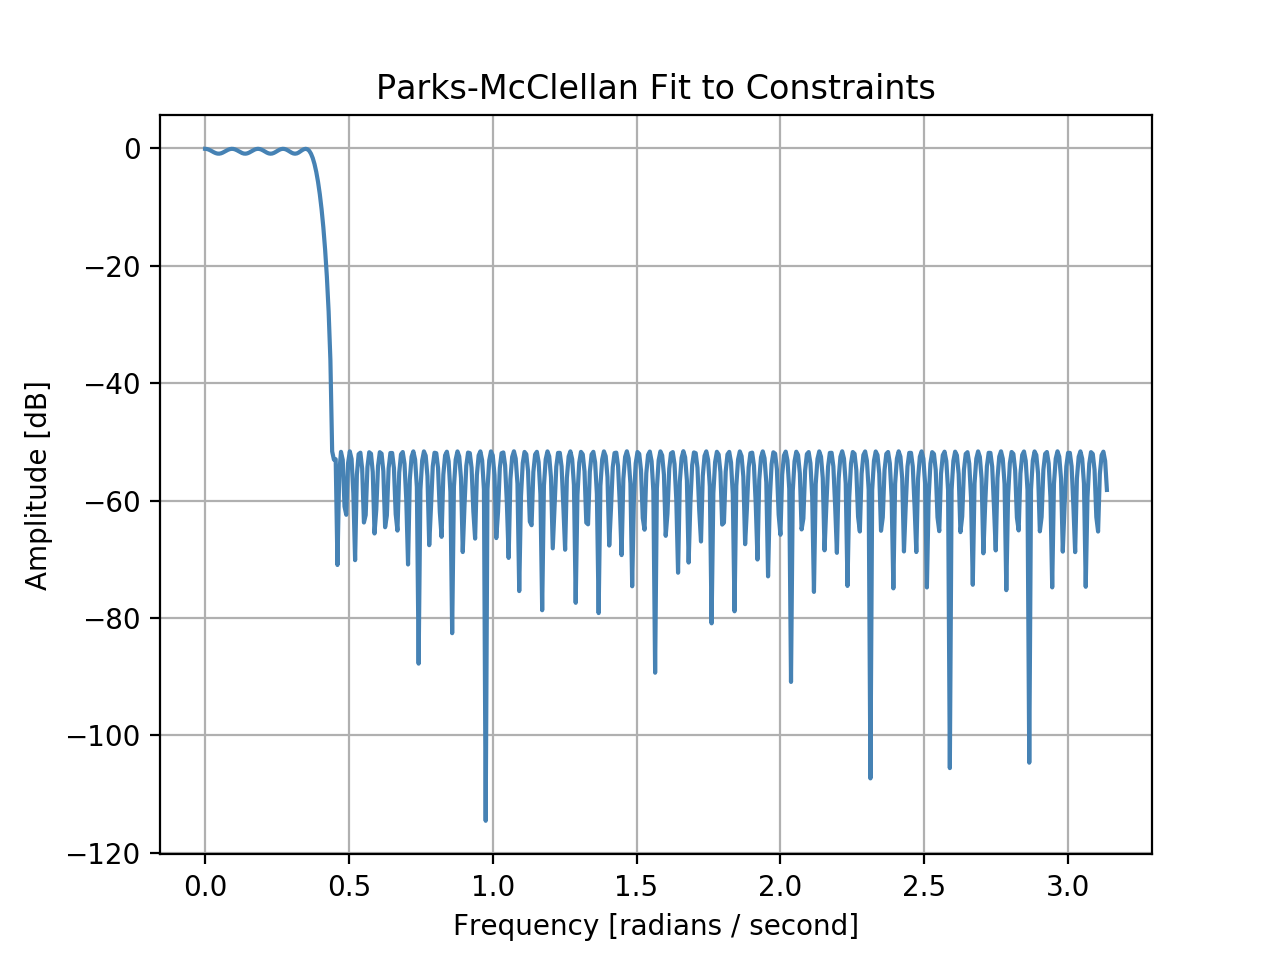
\includegraphics[width=.5\textwidth]{parks_2.png}
    \caption{This is the frequency response of the Parks-McClelland filter designed for the above specifications. This represents what I expect.}
\end{figure}

\begin{figure}[h] \label{fig:parks_2}
    \centering
    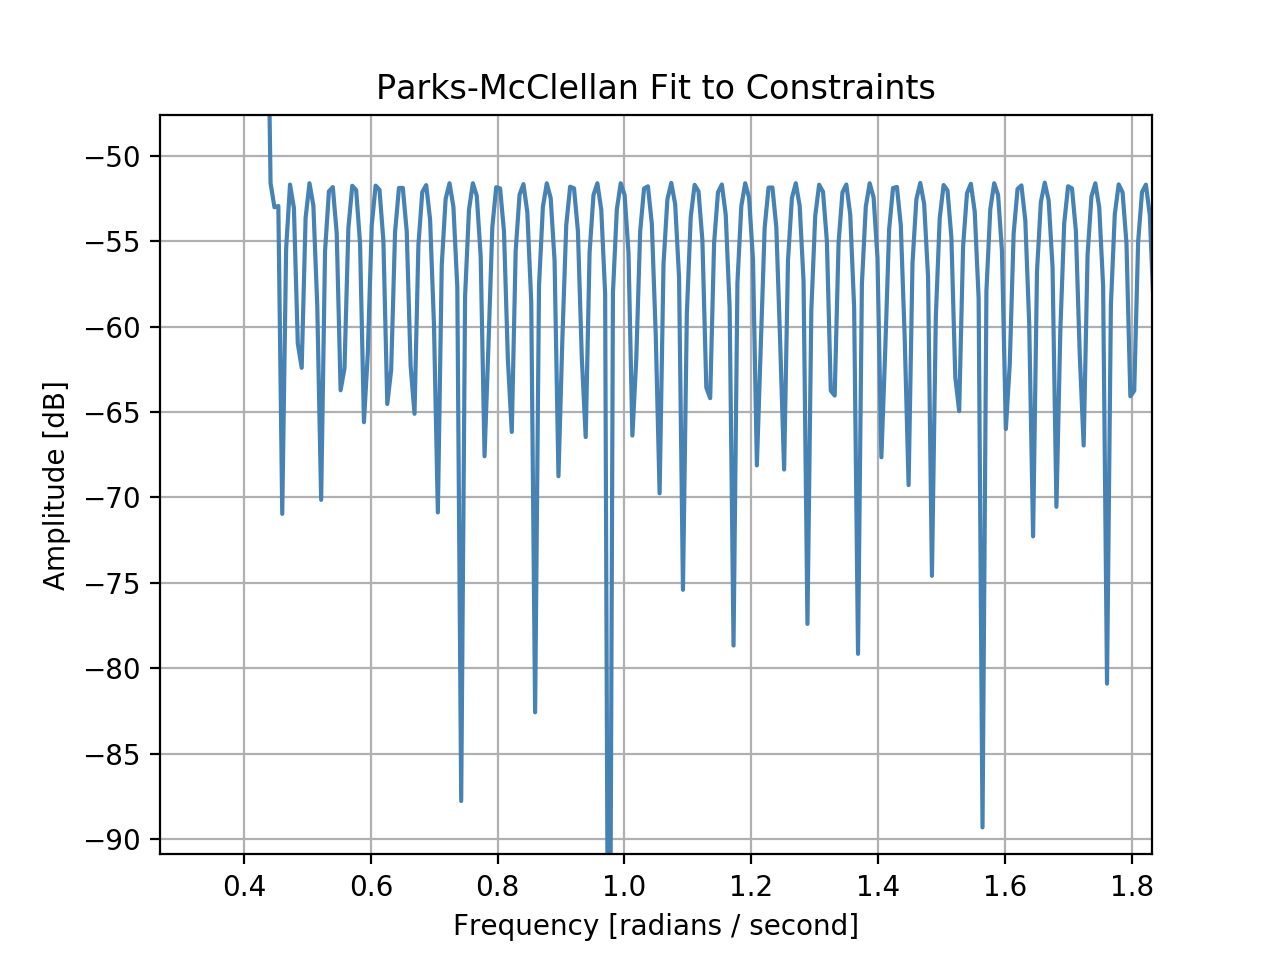
\includegraphics[width=.5\textwidth]{parks_2_3.png}
    \caption{This is the stopband of the frequency response of the Parks-McClelland filter designed for the above specifications. This represents what I expect.}
\end{figure}

\begin{figure}[h] \label{fig:parks_2}
    \centering
    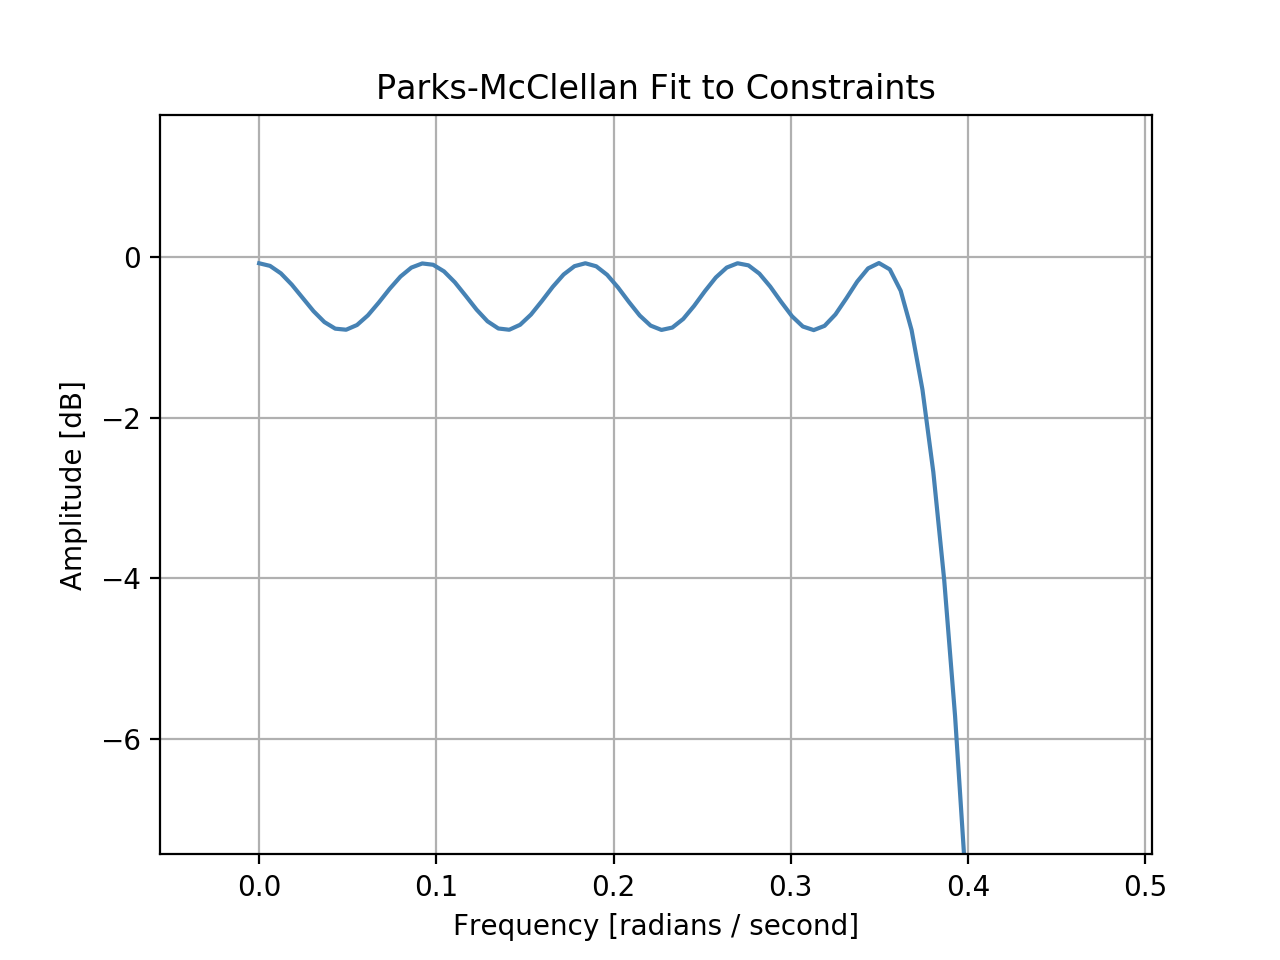
\includegraphics[width=.5\textwidth]{parks_2_1.png}
    \caption{This is the passband of the frequency response of the Parks-McClelland filter designed for the above specifications. This represents what I expect.}
\end{figure}

\begin{figure}[h] \label{fig:lowpass_2}
    \caption{}
    \centering
    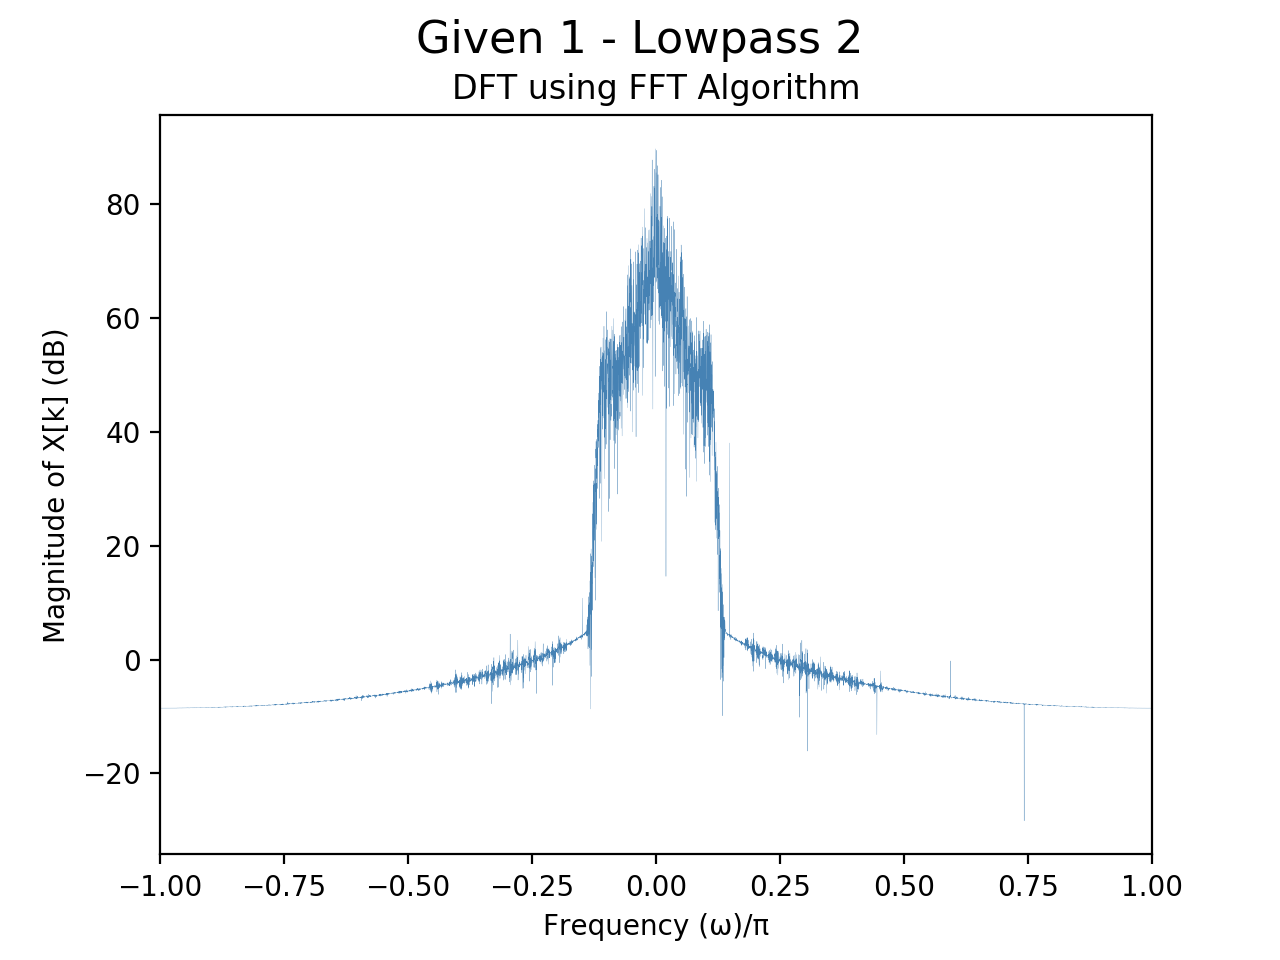
\includegraphics[width=.5\textwidth]{given_1_lowpass_2.png}
    \caption{This is the output DFT of the signal following the Parks-McClelland lowpass filter implementation.}
\end{figure}

\subsubsection{Decimation}

We complete decimation as above in Section~\ref{sec:downsampling_1} but with $M=4$. In other words, we took every fourth sample from the time-domain representation of the signal which is equivalent to decimation. Analysis of the DFT showed results which aligned with my expectations, as decimation produces frequency expansion. A second low pass filter could have been implemented, but that would have been a waste of computation time as the previous lowpass filter had a cutoff frequency below that necessary to prevent anti-aliasing. Our normalized discrete-time stopband frequency from the most previous lowpass filter was $\omega_{stop} = 36/256 \approx .1406 \leq .25$.

\begin{figure}[h] \label{fig:decimation}
    \caption{}
    \centering
    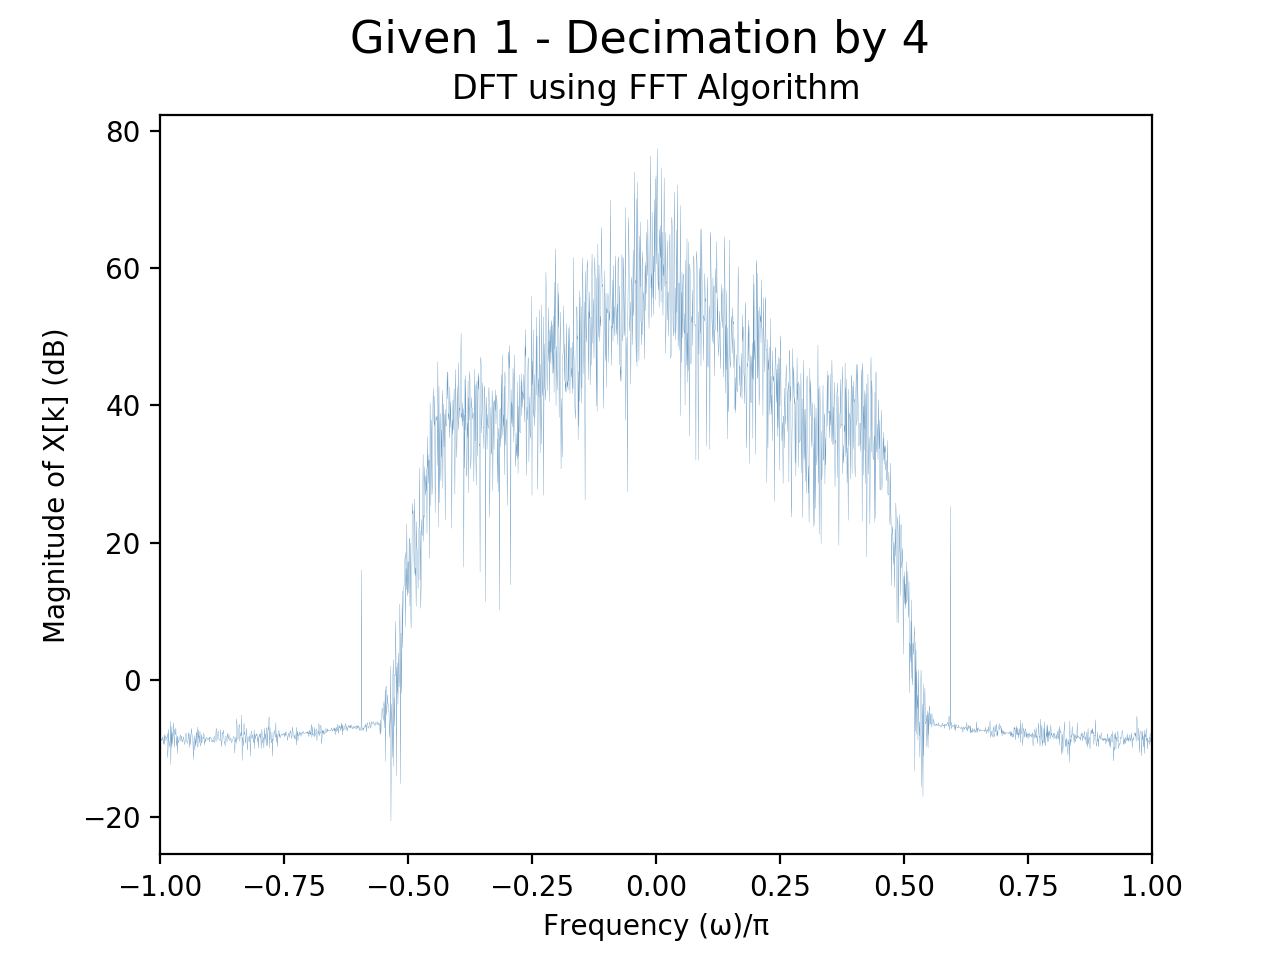
\includegraphics[width=.5\textwidth]{given_1_decimation_by_4.png}
    \caption{This plot show samples of the DTFT. This is following the decimation by 4 step. We see frequency expansion and, thus, this represents what I expect.}
\end{figure}

\subsection{Blind Test}

All three test files where analyzed as the sound quality was too exciting not to. I also analyzed my sound content as well.

\paragraph{Given Data 1} In this, we had a snip of the song "Wanted Dead or Alive" by Bon Jovi.

\paragraph{Given Data 2} In one of the sound bands, we had a classical piece followed by a description of the piece by the commentator.

\paragraph{Given Data 2} In this, we had a harsh guitar with a very enthusiastic man talking about rock music over the backing track.

\section{Code}

\subsection{Example Program using Class}

\begin{lstlisting}

# Given Signal 1 --------------------------------------------------------

# Load
given_1 = Signal.Signal(f_s, 100.6 * pow(10, 6), np.array([100 * pow(10, 3)]), 'gqrx_20191029_215237_100600000_2048000_fc.raw')

#Truncate to 10 seconds
given_1.truncate(20)
given_1.dft('Given 1 - Original Signal')

# # Modulate to baseband
given_1.modulate(0)
given_1.dft('Given 1 - Modulated')

# Lowpass Filter 8
M_1 = 8
Omega_s = f_s /(2 * M_1)
given_1.lowpass_chebII(Omega_s - (.1 * Omega_s), Omega_s)
given_1.dft('Given 1 - Chebyshev II Lowpass 1')

# Decimate
given_1.decimate(M_1)
given_1.dft('Given 1 - Decimation by 8')

# Discriminator
given_1.discriminator()
given_1.dft('Given 1 - Discriminator Output')

# Deemphasis
given_1.deemphasis(.000075) # 75 microsec
given_1.dft('Given 1 - Deemphasis Output')

# Lowpass at 15kHz
given_1.lowpass_parks(15 * pow(10, 3), 18 * pow(10, 3))
given_1.dft('Given 1 - Lowpass 2')

# Decimate
M_2 = 4
given_1.decimate(M_2)
given_1.dft('Given 1 - Decimation by 4')

# Confirm Data
given_1.play()

\end{lstlisting}

\subsection{Signal Class}

\begin{lstlisting}

import scipy
import scipy.signal as signal
import scipy.io.wavfile as wavf
from matplotlib import pyplot as plt
import numpy as np
import sounddevice as sd
import cmath
import time
import dtsp

class Signal:

	def __init__(self, f_s, Omega_c, Omega_0, file):
		# f_s = sampling frequency
		# W_c = hardware center frequency
		# w_0 = offsets of sound content
		# file = file name (string)

		print(" ---------------- INITIALIZING ---------------- ")

		self.f_s                 = f_s # sampling frequency
		self.Omega_c             = Omega_c # hardware center frequency
		self.Omega_0             = Omega_0 # array of offsets with sound content
		self.samples             = scipy.fromfile(open(file), dtype = scipy.complex64) # file name (string)
		self.data_length_sec     = self.samples.shape[0] / f_s
		self.data_length_samples = self.samples.shape[0]
		self.time_length         = int(.05 * self.f_s) # amount of time to plot
		self.color_1             = "steelblue"
		self.color_2             = "orange"
		self.color_3			 = "indianred"

		print("Data Length 0: {}".format(self.data_length_sec))

	def truncate(self, seconds):
		# seconds = length of signal in seconds

		print(" ---------------- TRUNCATE ---------------- ")

		self.data_length_samples = self.f_s * seconds # number of relevant points from data
		self.samples             = self.samples[0:self.data_length_samples] # truncate
		self.data_length_sec     = self.samples.shape[0] / self.f_s

		# print("Data Length: {}".format(self.data_length_sec))

	def dft(self, title):
		# Plot DFT of Samples through FFT Approximation

		print(" ---------------- DFT ---------------- ")
				# Look at Variables
		print("Length of input samples: {}".format(len(self.samples)))
		print("Samples: {}".format(self.samples))

		samples_dtft = np.fft.fft(self.samples) # fft of input samples
		N = len(samples_dtft) # Number of samples of the DTFT for the DFT

		fig, (ax1) = plt.subplots(1, 1)

		# Split Data (Positive Length)
		if N % 2 == 0:
			time_negative         = np.arange(int(-N/2), -1)
			time_positive         = np.arange(0, int(N/2) - 1)
			samples_dtft_positive = samples_dtft[0:int(N/2)-1]
			samples_dtft_negative = samples_dtft[int(N/2):N-1]
		else:
			time_negative         = np.arange(int(-(N/2) + .5), -1)
			time_positive         = np.arange(0, int((N/2) - .5))
			samples_dtft_positive = samples_dtft[0 : int((N/2) - .5)]
			samples_dtft_negative = samples_dtft[int((N/2) + .5): N-1]

		# Plot Magnitude
		factor = 500
		fig.suptitle(title, fontsize=16)
		ax1.plot(2*time_positive[::factor]/N, 20*np.log10(np.abs(samples_dtft_positive[::factor])), linewidth=0.1,  color = self.color_1) # magnitude
		ax1.plot(2*time_negative[::factor]/N, 20*np.log10(np.abs(samples_dtft_negative[::factor])), linewidth=0.1,  color = self.color_1) # magnitude
		ax1.set_xlabel('Frequency (\u03C9)/\u03C0')
		ax1.set_ylabel('Magnitude of X[k] (dB)')
		ax1.set_xlim([-1, 1])
		ax1.set_title('DFT using FFT Algorithm')
		plt.show()

		# Look at Variables
		# print("Length of input samples: {}".format(len(self.samples)))
		# print("Samples: {}".format(samples_dtft[0:int(N/2)]))
		# print("Length of dft: {}".format(N))
		# print("Length of time_positive: {}".format(len(time_positive)))
		# print("First Sample: {}".format(samples_dtft[0]))
		# print("Last Sample: {}".format(samples_dtft[-1]))
		# print("Last Sample: {}".format(samples_dtft[N-1]))

	def modulate(self, index):

		print(" ---------------- MODULATE ---------------- ")

		omega_0 = 2 * np.pi * self.Omega_0[index] / self.f_s # solve for discrete time modulation frequency
		modulating_function = np.exp(-1j * omega_0 * np.arange(self.data_length_samples))
		self.samples = self.samples * modulating_function # modulate

		# Look at Variables
		# print("omega_0: {}".format(omega_0))
		# print("Modulating Function: {}".format(modulating_function))
		# print("Omega: {}".format(self.Omega_0[index]))
		# print("Samples: {}".format(self.samples))
		# print("Vector of n: {}".format(np.arange(self.data_length)))

	def lowpass_chebII(self, Omega_p, Omega_s):

		# Omega_p (Hz) 
		# Omega_s (Hz)

		print(" ---------------- LOWPASS FILTER CHEB II ---------------- ")

		# Initialize IIR Parameters ------------------------------

		omega_p     = (2 * Omega_p) / self.f_s # normalized band
		omega_s     = (2 * Omega_s) / self.f_s # normalized band
		max_gain_p  = 0 # dB
		min_atten_p = 1 # dB
		ripple_p    = min_atten_p - max_gain_p # dB
		max_atten_s = 50 # dB

		# Generate Filter Parameters
		ord, ws = signal.cheb2ord(omega_p, omega_s, min_atten_p - max_gain_p, max_atten_s)

		# Outputs polynomial coefficients, using the bilinear transform automatically
		b, a = signal.cheby2(ord, max_atten_s, ws, output='ba')

		# Plot Frequency Response
		w, h = signal.freqz(b, a)
		plt.plot(w, 20 * np.log10(abs(h)), color = self.color_1)
		# print(20 * np.log10(abs(h)))
		plt.title('Chebyshev II Fit to Constraints')
		plt.xlabel('Frequency [radians / second]')
		plt.ylabel('Amplitude [dB]')
		plt.grid(which='both', axis='both')
		plt.show()

		sos = signal.cheby2(ord, max_atten_s, ws, output='sos')
		self.samples = signal.sosfilt(sos, self.samples)

		print("Chebyshev II Parameters: \na = {} \nb = {} \nord ={} ".format(a,b,ord))
		print("omega_p: {}".format(omega_p))
		print("omega_s: {}".format(omega_s))

	def lowpass_parks(self, Omega_p, Omega_s):

		print(" ---------------- LOWPASS FILTER PARKS-MCCLELLAND ---------------- ")

		k       = (10**(-1/20) + 1) / 2
		dpass   = (1/k) - 1
		dstop   = 1/(100 * k * np.sqrt(10))

		omega_p = (2 * Omega_p) / self.f_s # normalized band
		omega_s = (2 * Omega_s) / self.f_s # normalized band

		print("dpass: {}".format(dpass))
		print("dstop: {}".format(dstop))
		print("omega_p: {}".format(omega_p))
		print("omega_s: {}".format(omega_s))

		numtaps, bands, amps, weights = dtsp.remezord([omega_p/2.0, omega_s/2.0], [1, 0], [dpass,dstop], Hz=1)
		bands *= 2.0    # above function outputs frequencies normalized from 0.0 to 0.5

		print("numtaps: {}".format(numtaps))

		b = signal.remez(numtaps, bands, amps, weights, Hz=2.0)
		
		print("Parks-McClellan Parameters: \nb = {} \nk = {}".format(b, k))
		print("Length b: {}".format(b.shape))

		# Plot Frequency Response
		w, h = signal.freqz(k*b)
		plt.plot(w, 20 * np.log10(abs(h)), color = self.color_1)
		# print(20 * np.log10(abs(k*h)))
		plt.title('Parks-McClellan Fit to Constraints')
		plt.xlabel('Frequency [radians / second]')
		plt.ylabel('Amplitude [dB]')
		plt.grid(which='both', axis='both')
		plt.show()

		# self.samples = signal.filtfilt(k * b, [1], self.samples)
		self.samples = signal.lfilter(k * b, [1], self.samples)

	def downsample(self, factor):

		# Use pre-built filter for AA and decimate
		self.samples             = scipy.signal.decimate(self.samples, factor)
		self.f_s                 = self.f_s / factor
		self.data_length_sec     = self.samples.shape[0] / self.f_s
		self.data_length_samples = self.samples.shape[0]
		self.time_length         = int(1 * self.f_s) # amount of time to plot

		# Look at Variables
		print("Data Length: {}".format(self.data_length_samples))
		print("Shape {}".format(self.samples.shape[0]))
		print("f_s {}".format(self.f_s))

	def decimate(self, factor):

		print(" ---------------- DECIMATE ---------------- ")

        # Downsample
		self.samples             = self.samples[::factor] # downsample
		self.f_s                 = self.f_s / factor # update f_s
		self.data_length_sec     = self.samples.shape[0] / self.f_s # update total length of data in sec
		self.data_length_samples = self.samples.shape[0] # update total number of samples
		self.time_length         = int(1 * self.f_s) # amount of time to plot

		# Look at Variables
		# print("Downsample by 8 Samples: {}".format(self.samples))
		print("Length of input samples: {}".format(self.data_length_samples))

	def discriminator(self):

		print(" ---------------- DISCRIMINATOR ---------------- ")

		samples = self.samples # save vector before filtering

		# Limiter ------------------------------------------------
		y_1 = self.samples / np.abs(self.samples) # normalize amplitude

		# DT Differentiator --------------------------------------
		M       = 5 # filter length
		beta    = 2.4 # Kaiser parameter
		n       = np.arange(0, M+1) # time vector
		h_ideal = ((np.cos(np.pi * (n - (M/2))) / (n - (M/2))) - (np.sin(np.pi * (n - (M/2))) / (np.pi * ((n - (M/2)) ** 2)))) # ideal impulse response
		h_ideal = h_ideal[0:M+1] # segmented ideal response
		w       = signal.kaiser(M + 1, beta) # windowing function
		h       = h_ideal * w # windowing data
		y_1a    = signal.convolve(h, y_1) # x * h convolution to differentiate data

		# Conjugate ---------------------------------------------
		y_1b = np.conj(y_1) 

		# Non-integer Delay -------------------------------------
		h_nid = np.sinc(n - M/2)
		y_1b  = signal.convolve(h_nid, y_1b)

		# Multiplication in Time --------------------------------
		y_1b = y_1b[0:y_1a.shape[0]]
		y_2  = y_1a * y_1b

		# Imaginary ---------------------------------------------
		self.samples             = np.imag(y_2)
		self.data_length_sec     = self.samples.shape[0] / self.f_s # update total length of data in sec
		self.data_length_samples = self.samples.shape[0] # update total number of samples

		print("self.samples: {}".format(self.samples))

		# Plot Impulse ------------------------------------------
		fig, (ax1, ax2, ax3) = plt.subplots(3, 1)
		fig.suptitle('Discrete-time Differentiator', fontsize=16)

		# Ideal
		ax1.stem(n, h_ideal, use_line_collection=True)
		ax1.set_xlabel('Sample Number (n)')
		ax1.set_ylabel('Amplitude')
		ax1.set_title("Truncated Ideal Differentiator Impulse Response, h[n]")

		ax2.stem(n, w, use_line_collection=True)
		ax2.set_xlabel('Sample Number (n)')
		ax2.set_ylabel('Amplitude')
		ax2.set_title("Kaiser Windowing Function, w[n]")

		ax3.stem(n, h, use_line_collection=True)
		ax3.set_xlabel('Sample Number (n)')
		ax3.set_ylabel('Amplitude')
		ax3.set_title("Windowed Impulse Response, w[n]h[n]")
		
		plt.show()

		# Plot Signal Change ------------------------------------
		fig = plt.figure()
		fig.suptitle('Signal Before and After the Discriminator', fontsize=16)
		
		plt.plot(np.arange(0, self.time_length)/self.f_s, samples[0:self.time_length], color = self.color_1) # magnitude
		plt.plot(np.arange(0, self.time_length)/self.f_s, self.samples[0:self.time_length], color = self.color_2) # magnitude
		plt.xlabel('Time (sec)')
		plt.ylabel('Amplitude')
		plt.xlim([0, 1])
		plt.legend(['Before Discriminator', 'After Discriminator'])

		# Look at Variables
		# print("y_1a: {}".format(y_1a))		
		# print("h: {}".format(h))
		# print("n: {}".format(n))
		# print("h_ideal: {}".format(h_ideal))
		# print("window: {}".format(w))
		# print("y_1: {}".format(y))
		# print("Data Length: {}".format(self.data_length_sec))
		# print("Shape {}".format(self.samples.shape[0]))
		# print("Time Shift: {}".format(time_shift))
		# print("y_1b: {}".format(y_1b))
		# print("y_1a shape: {}".format(y_1a.shape[0]))
		# print("y_2: {}".format(y_2))

	def deemphasis(self, tau_d):

		print(" ---------------- DEEMPHASIS FILTER ---------------- ")

		samples = self.samples # save vector before filtering

        # Define Continuous-time Filter ------------------------
		b    = np.array([1])
		a    = np.array([tau_d, 1])
		w, h = signal.freqs(b, a)

		# Plot
		plt.plot(w, 20 * np.log10(abs(h)), color = self.color_1)
		plt.title('H_d(j\u03A9)')
		plt.xlabel('Frequency [1 / second]')
		plt.ylabel('Magnitude [dB]')
		plt.grid(which = 'both', axis = 'both')
		plt.show()

		# Bilinear Transform -----------------------------------
		b_transform, a_transform = signal.bilinear(b, a, self.f_s)

		# Plot
		w_transform, h_transform = signal.freqz(b_transform, a_transform)
		plt.plot(w_transform, 20 * np.log10(abs(h_transform)), color = self.color_1)
		plt.title('Bilinear Transform of H_d(j\u03A9)')
		plt.xlabel('Frequency [radians / second]')
		plt.ylabel('Magnitude [dB]')
		plt.grid(which = 'both', axis = 'both')
		plt.show()

		# Filter Signal -----------------------------------------
		self.samples = signal.lfilter(b_transform, a_transform, self.samples)

		# Plot Signal Change ------------------------------------
		fig = plt.figure()
		fig.suptitle('Signal Before and After the Deemphasis', fontsize=16)
		
		plt.plot(np.arange(0, self.time_length)/self.f_s, samples[0:self.time_length], color = self.color_1) # magnitude
		plt.plot(np.arange(0, self.time_length)/self.f_s, self.samples[0:self.time_length], color = self.color_2) # magnitude
		plt.xlabel('Time (sec)')
		plt.ylabel('Amplitude')
		plt.xlim([0, 1])
		plt.legend(['Before Deemphasis', 'After Deemphasis'])

		# View Variables
		# print("num: {}\nden: {}".format(b_transform, a_transform))
		# print("Pole Zero: {}".format(signal.tf2zpk(b, a)))

	def play(self):

		sd.play(self.samples, self.f_s)
		time.sleep(20)
		sd.stop()

\end{lstlisting}


\end{document}
